\chapter{骨科相关感染的自动诊断与可视化方法}

第三章和第四章分别详细地介绍了应用于动态骨显像和PET/CT中以人工智能为基础的假体关节感染辅助诊断框架和骨折相关感染辅助检测诊断框架。由于这两个框架无法提供便利且直观的辅助诊断以及可视化,本章继续在这一研究方向上深入,结合这两种人工智能方法并采用最新的PyQt6框架,去设计一种新颖的骨科相关感染的自动诊断与可视化方法。该方法旨在构建一个骨科相关感染的自动辅助诊断系统,提供全面的医学影像可视化、阅览和分析功能,以促进临床诊断中假体关节感染与骨折相关感染的诊断决策和提高准确性。

\section{问题分析}

在设计假体关节感染和骨折相关感染的自动诊断与可视化方法时,必须深入考虑核医学专家在诊断这类骨科相关感染疾病的具体流程和对医学影像的可视化需求。这一方法需要融合多种先进的图像处理技术,同时也要求透彻地理解并仿真医生的诊断流程。这要求此方法不仅要精确处理和展示医学影像,还具备医学的决策智能,以提供直观、准确的诊断辅助。因此,本章主要包含以下两个方面的研究:

(1)\textbf{模拟核医学医生的诊断流程。}在假体关节感染和骨折相关感染诊断任务中,核医学专家遵循的实际临床诊断流程具体包括:首先,在动态骨显像或PET/CT中,精确定位到潜在的病灶区域。随后,核医学专家依靠专业的工具对所定位的病灶区域进行深入的分析和评估。最后,核医学专家将依托其丰富的临床经验和细致的视觉评估作出最终的诊断决策。

由此,在本章中,所研究的自动诊断方法需要集成第三章和第四章设计的图像处理技术。这些图像处理技术能够从复杂的动态骨显像和PET/CT影像中提取到关键的生物标志物,通过端到端地方式直接在医学影像中进行辅助诊断。特别是第三章采用了CNN和ConvLSTM,用于深入地学习动态骨显像中的图像特征和序列变化,这对于髋关节和膝关节假体感染的准确诊断至关重要。同时,第四章利用基于深度学习的检测和分类算法处理PET/CT影像,以获得更加全面立体的解剖结构和生理代谢信息,进而有效地锁定病灶区域,并对骨折相关感染进行精准诊断。

(2)\textbf{不同医学影像模态的可视化。}在核医学专家的临床诊断流程中,不同医学影像的可视化是最基础的需求之一。可视化需要能够处理、解析和展示不同来源的影像数据,如动态骨显像和PET/CT(PET SUV和CT HU),保证医生在做出诊断决策时能够全面考量所有相关影像信息。

由此,在本章中,所研究的可视化方法需要使得医学影像可根据专业医生的具体需求进行个性化调整,包括调整对比度、缩放、以及使用不同的着色模型以适应不同的医学影像模态和增强特定组织或病变的可视性等。同时,也需要特别注重和优化医生的视觉体验,提供直观的用户界面来展示各种各样的影像数据。通过提供分层视图、切换视图、融合影像和三维重建功能等,帮助医生从不同角度分析单一模态和多模态影像,从而得到更全面的诊断信息。

\section{总体设计}

\begin{figure}[h]
  \centering
  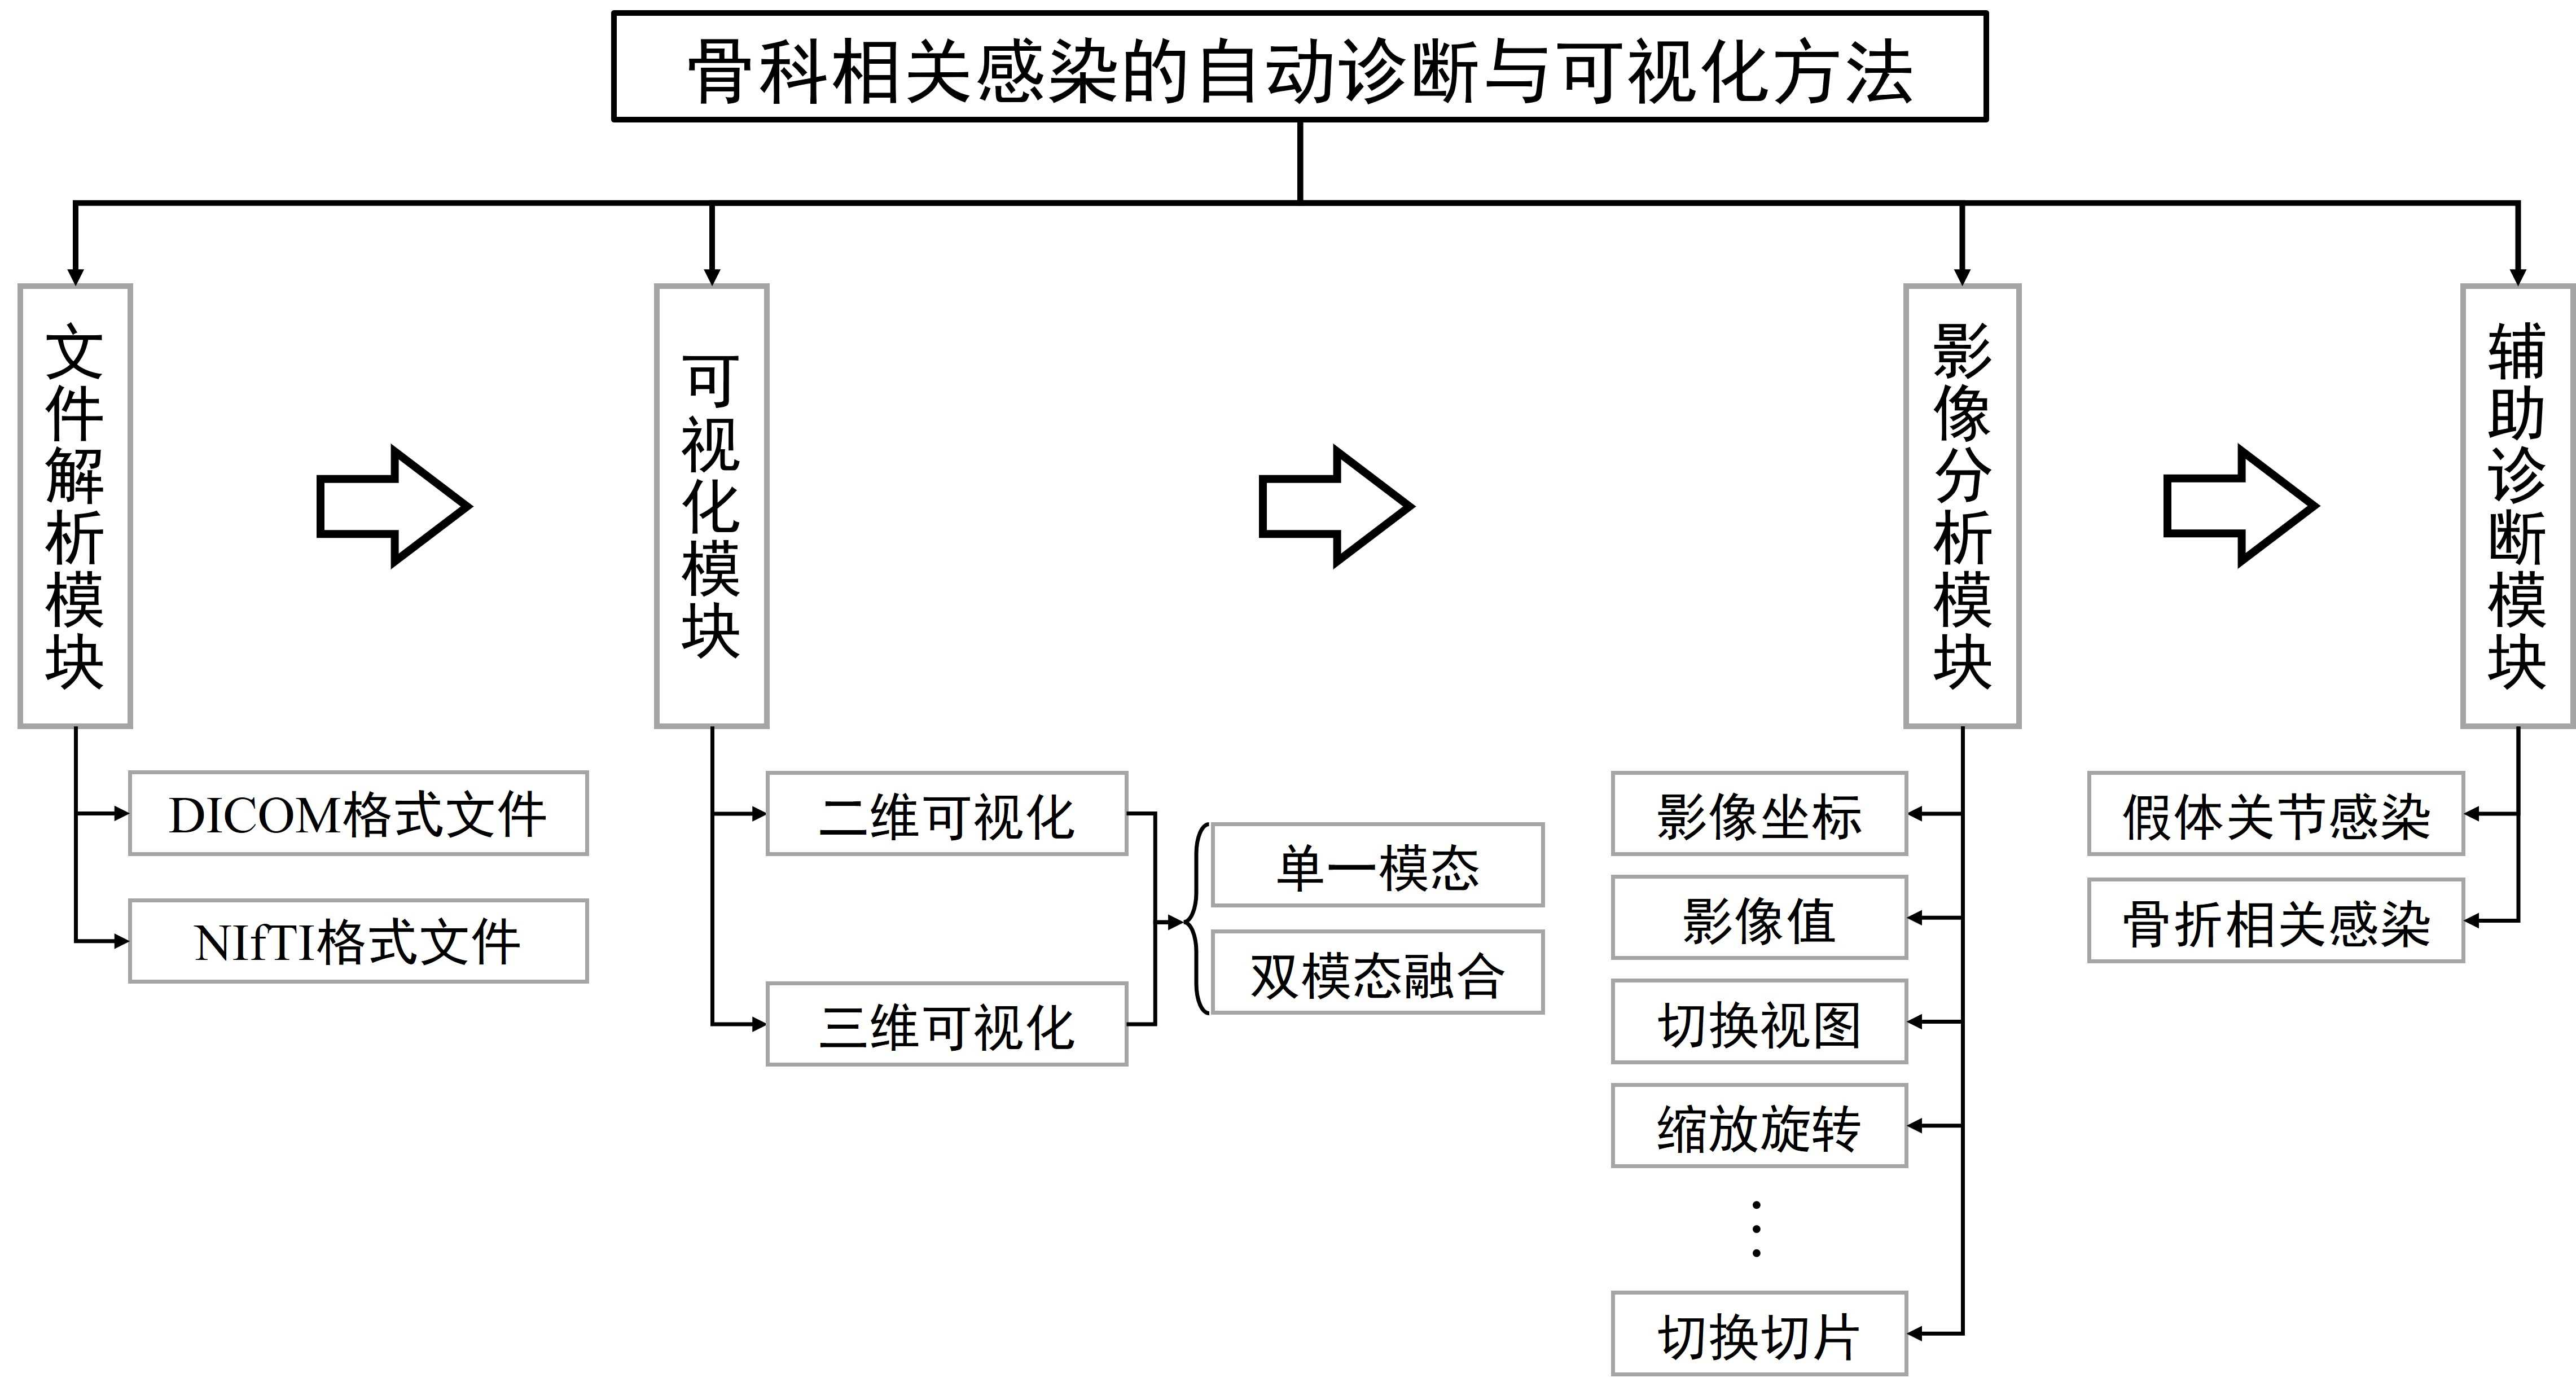
\includegraphics[width=\textwidth]{figures/chap05_overall.jpg}
  \caption{骨科相关感染的自动诊断与可视化方法的总体设计图}
  \label{fig:chap05_overall}
\end{figure}

本章设计了一个基于深度学习和PyQt6框架的骨科相关感染自动诊断和可视化方法,旨在提供精确地诊断辅助。如图\ref{fig:chap05_overall}所示的方法流程涵盖了四个关键模块和相应的操作流程。整个方法流程由四个主要步骤构成:
\begin{enumerate}
  \item \textbf{文件解析}:被用户选定的DICOM或NIfTI文件经过读取和解析,其中根据各自的文件规范执行相应的解码流程,旨在准确抽取所需的医学信息数据。
  \item \textbf{可视化}:经过解析得到的数据在预处理后转化为视觉表现形式,以直观展示医学影像。该预处理包括标准化、配准和融合,以提供丰富且细致的视觉信息。
  \item \textbf{影像分析}:在实现影像数据的视觉呈现后,影像分析步骤提供了一系列工具,用于在多个视角和尺度下观察医学影像,包括视图切换、仿射变换等等操作。
  \item \textbf{辅助诊断}:在用户通过可视化和影像分析获得初步印象后,辅助诊断步骤通过第三章和第四章中描述的深度学习框架,为假体关节感染和骨折相关感染提供辅助诊断能力。
\end{enumerate}

从文件解析开始,DICOM和NIfTI格式的医学影像数据由文件解析模块进行读取与解析。DICOM数据由于其独有的详细性和医疗信息的丰富性,需要处理其复杂的元数据以提取诊断所需的重要数据;而NIfTI格式则常用于功能成像和三维影像处理,因此其解析旨在获取空间结构信息以便后续分析。

在完成解析之后,可视化模块将根据用户选择的医学影像数据和可视化功能进行相应的处理操作。该模块支持单模态和双模态影像的二维和三维可视化。在可视化过程中,医学影像数据均被默认设置为三维结构。对于原本是二维的医学影像数据,将自动扩展出一个大小为一的维度,以便与既定的三维数据结构保持一致性。因此,本章可视化模块的数据处理和分析侧重于三维及以下维度的医学影像。

影像分析模块根据用户的个性化需求,对医学影像执行特定的操作。此模块涵盖的功能颇为广泛,包括展示影像坐标与在特定坐标上用于临床评估的影像值、切换不同视图,例如矢状面、冠状面和横断面、以及执行如平移、缩放、旋转这样的仿射变换操作等。每项功能都旨在为医生提供详细的医学影像信息,从而更准确地定位和诊断潜在的病灶区域。

最终,在完成医学影像的可视化以及初步分析后,辅助诊断模块融合了假体关节感染辅助诊断框架与骨折相关感染检测诊断框架,可以给用户提供医学辅助诊断建议。该建议包括在动态骨显像中对患者的膝部或髋部的假体进行诊断,以及利用PET/CT影像检测与识别患者下肢中潜在的感染区域。辅助诊断模块基于医学影像特征辅助医生评估病灶的性质以及严重程度,为医学诊断提供更高的准确性与效率。

\subsection{界面设计}

\begin{figure}[htbp]
  \centering
  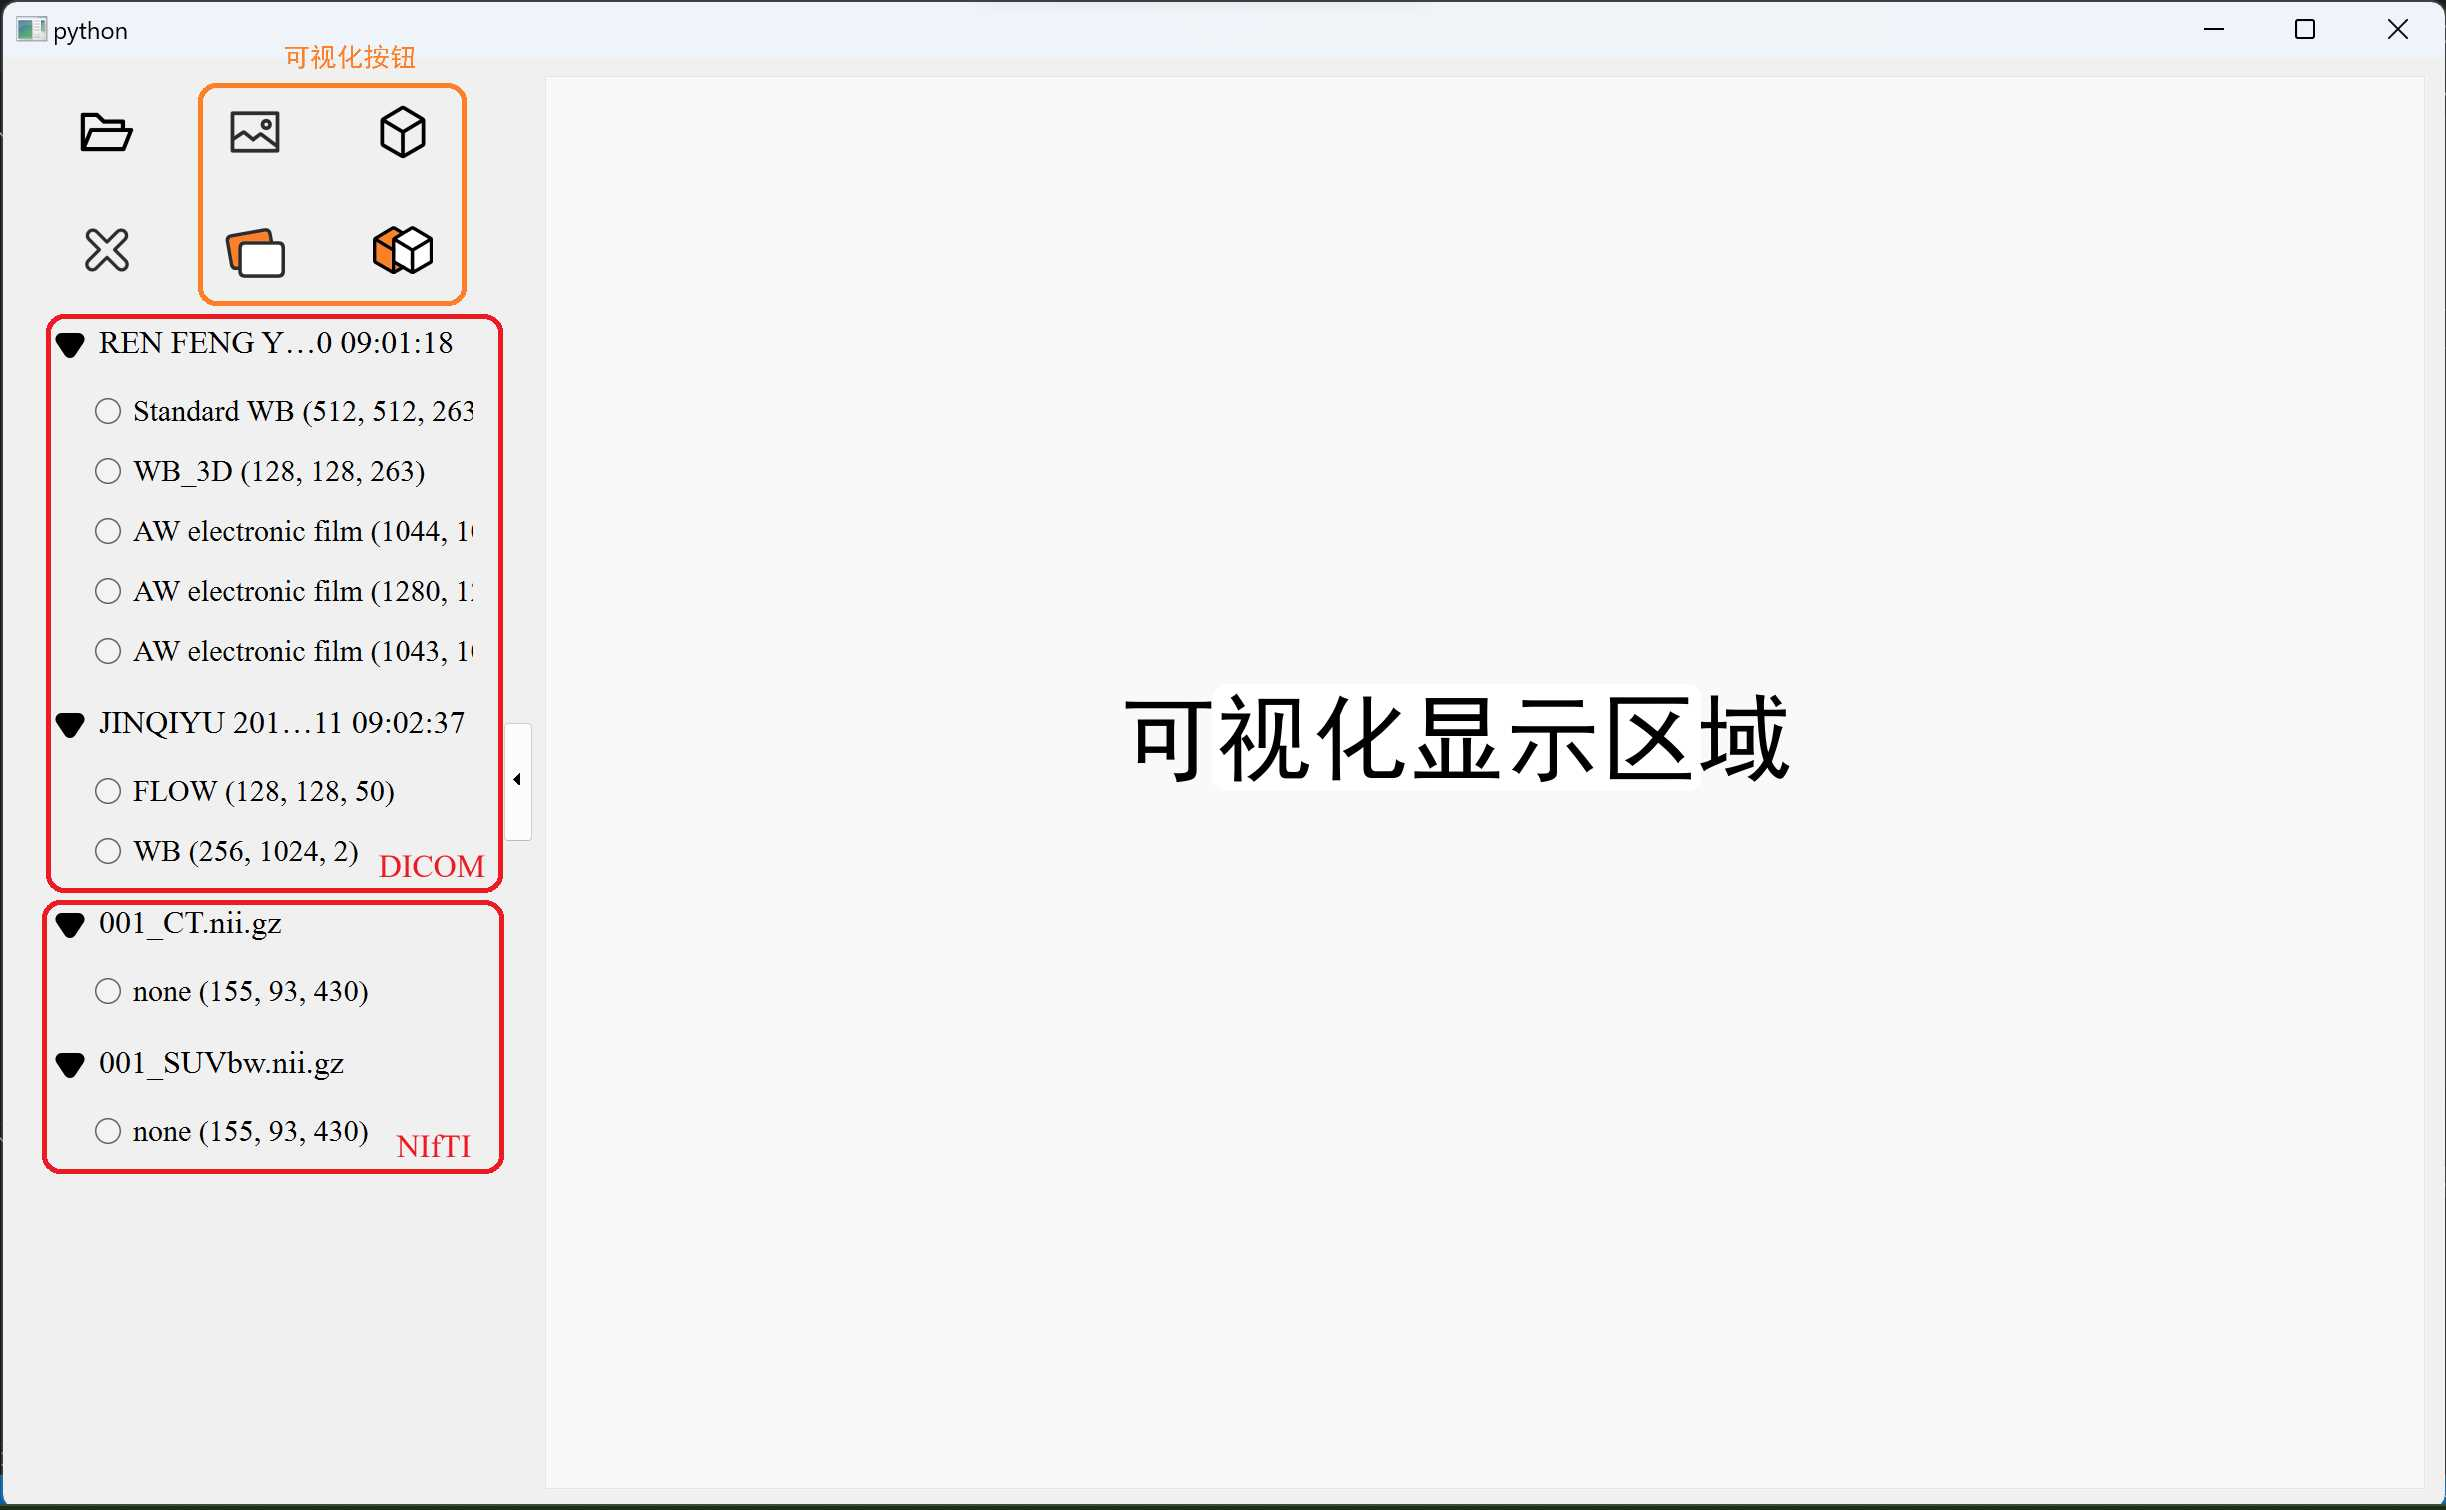
\includegraphics[width=\textwidth]{figures/chap05_preview.jpg}
  \caption{骨科相关感染的自动辅助诊断系统界面}
  \label{fig:chap05_preview}
\end{figure}

图\ref{fig:chap05_preview}呈现的是所设计的骨科相关感染自动化辅助诊断系统的界面。界面主要分为侧边导航栏和中心的可视化显示区域。在侧边导航栏中,展示了DICOM和NIfTI文件由文件解析模块处理所得的层次化结构信息。该信息采用了可折叠的列表按钮的形式,详细地列出了患者的姓名拼音与影像扫描的具体时间,并在其内部展示了归属于当前患者的影像数据,例如系列描述与影像尺寸信息。侧边栏顶部设置了多个功能按钮,包括打开文件、删除已解析的影像数据、二维影像展示、三维影像展示、二维影像融合以及三维影像融合。其中,功能按钮将作用于侧边导航栏中被勾选的医学影像数据。

中央的可视化显示区域将依据操作者在侧边导航栏中执行的操作,以标签页的形式对医学影像数据进行可视化显示。图\ref{fig:chap05_view}展示了四种不同可视化功能下每个标签页顶部配备的工具栏,其中融合了影像分析模块与辅助诊断模块的众多功能。

\begin{figure}[htbp]
  \centering
  \subfloat[二维展示]{
    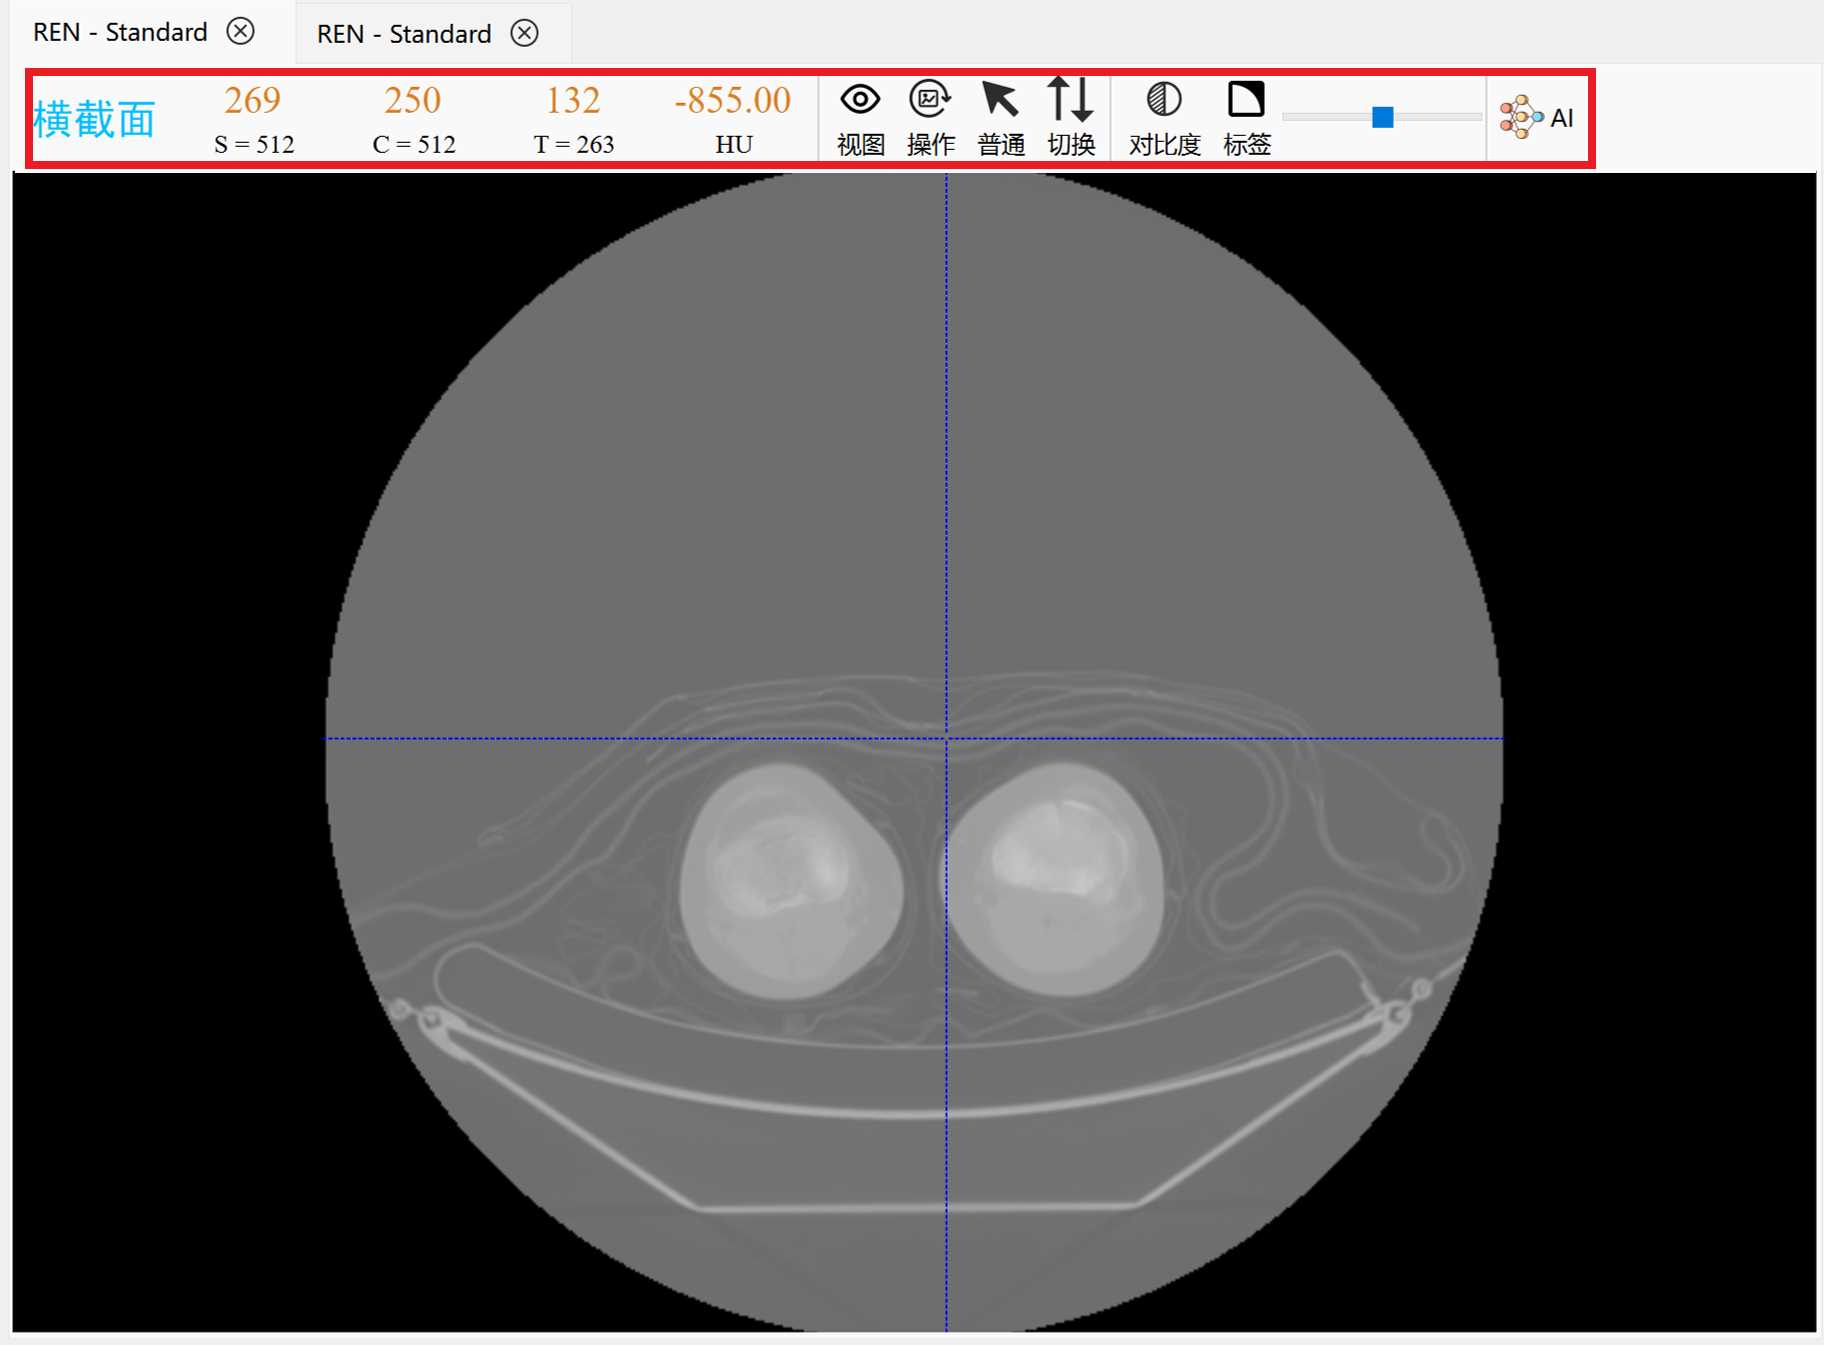
\includegraphics[width=0.49\textwidth]{figures/chap05_view_2D.jpg}
    \label{fig:chap05_view_2D}
  }
  \subfloat[二维融合]{
    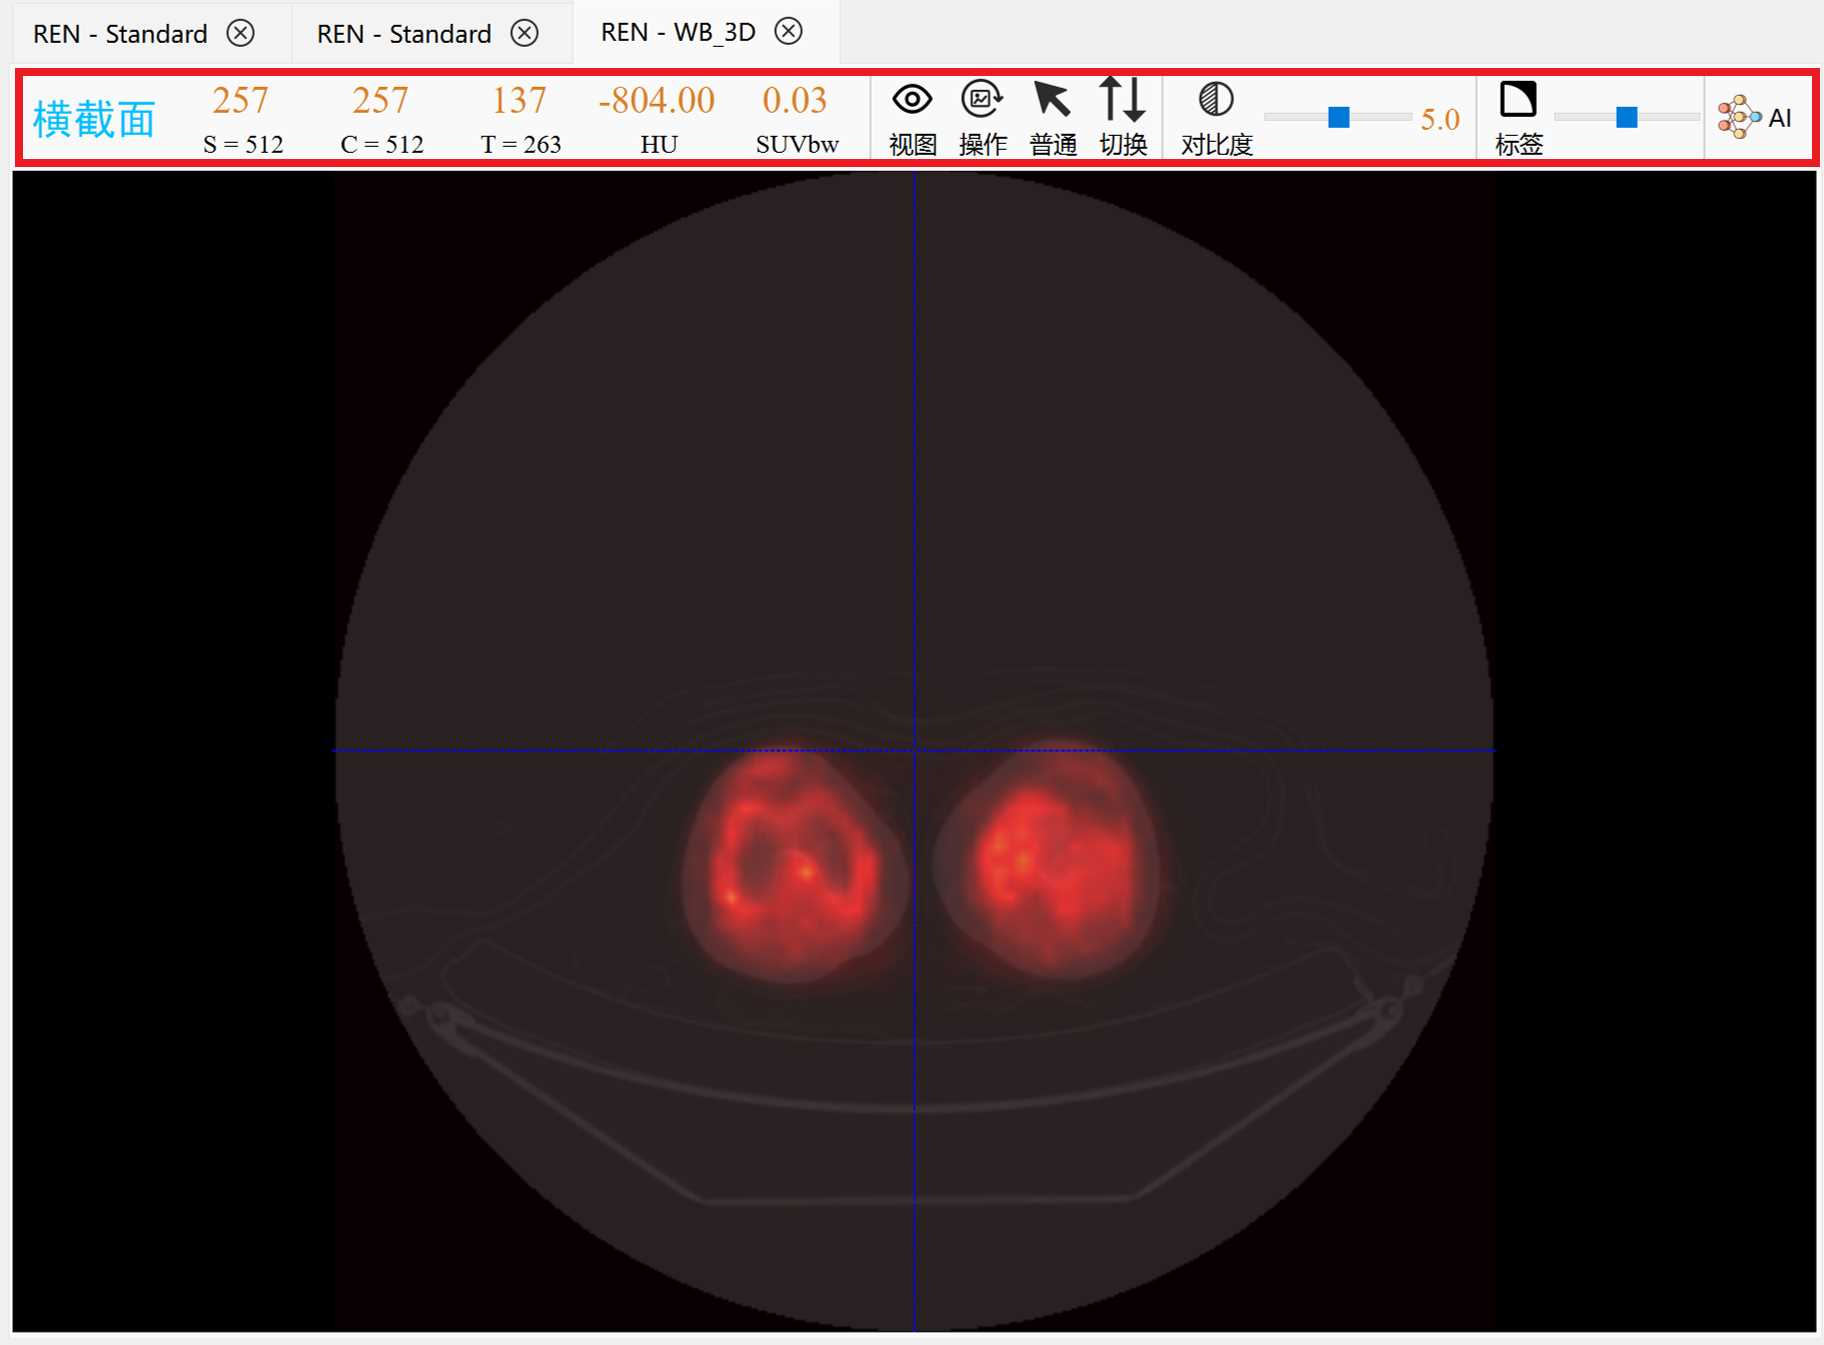
\includegraphics[width=0.49\linewidth]{figures/chap05_view_2DF.jpg}
    \label{fig:chap05_view_2DF}
  }
  \newline
  \newline
  \subfloat[三维展示]{
    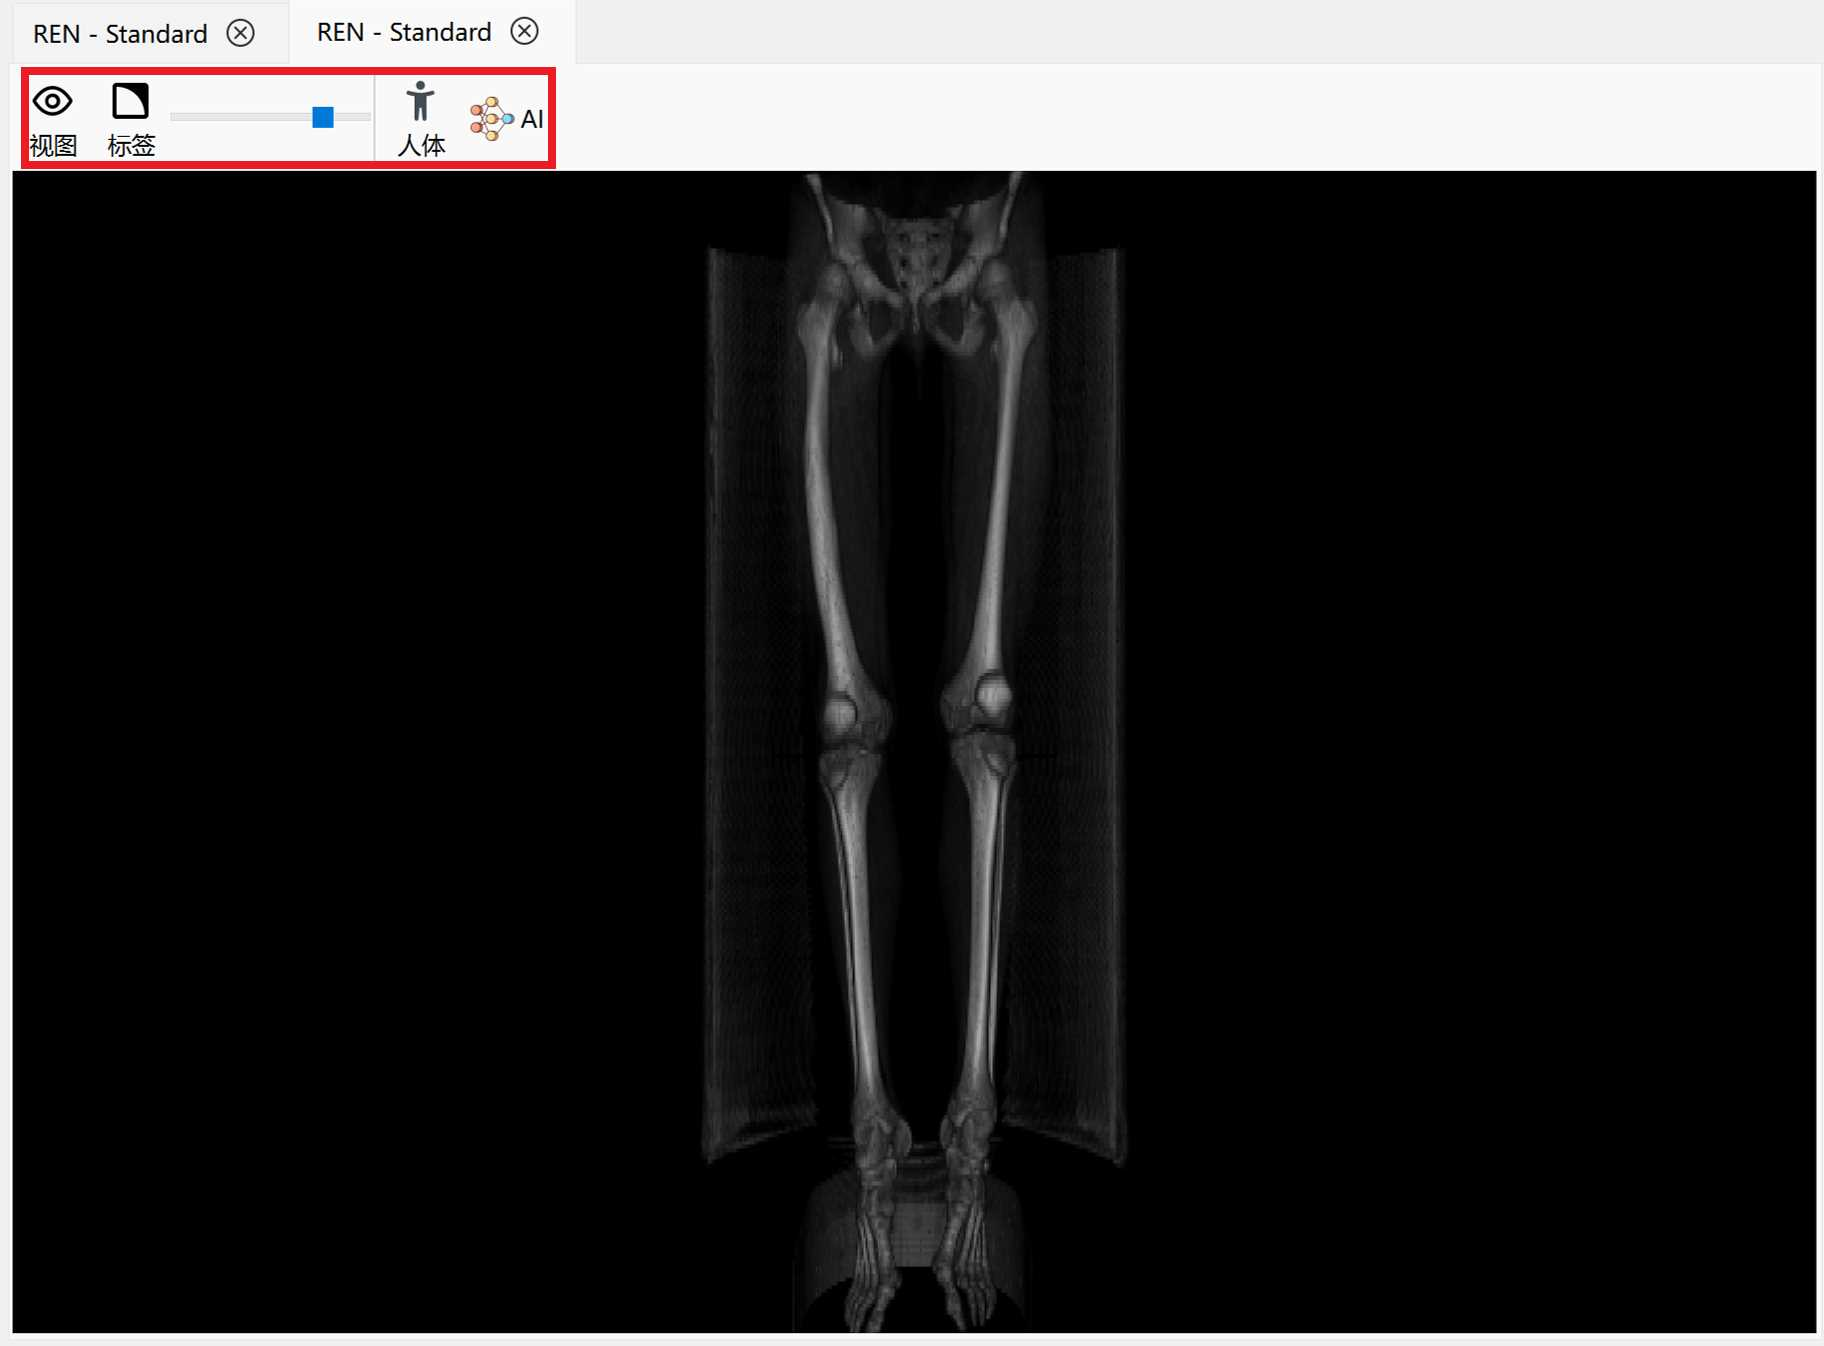
\includegraphics[width=0.49\linewidth]{figures/chap05_view_3D.jpg}
    \label{fig:chap05_view_3D}
  }
  \subfloat[三维融合]{
    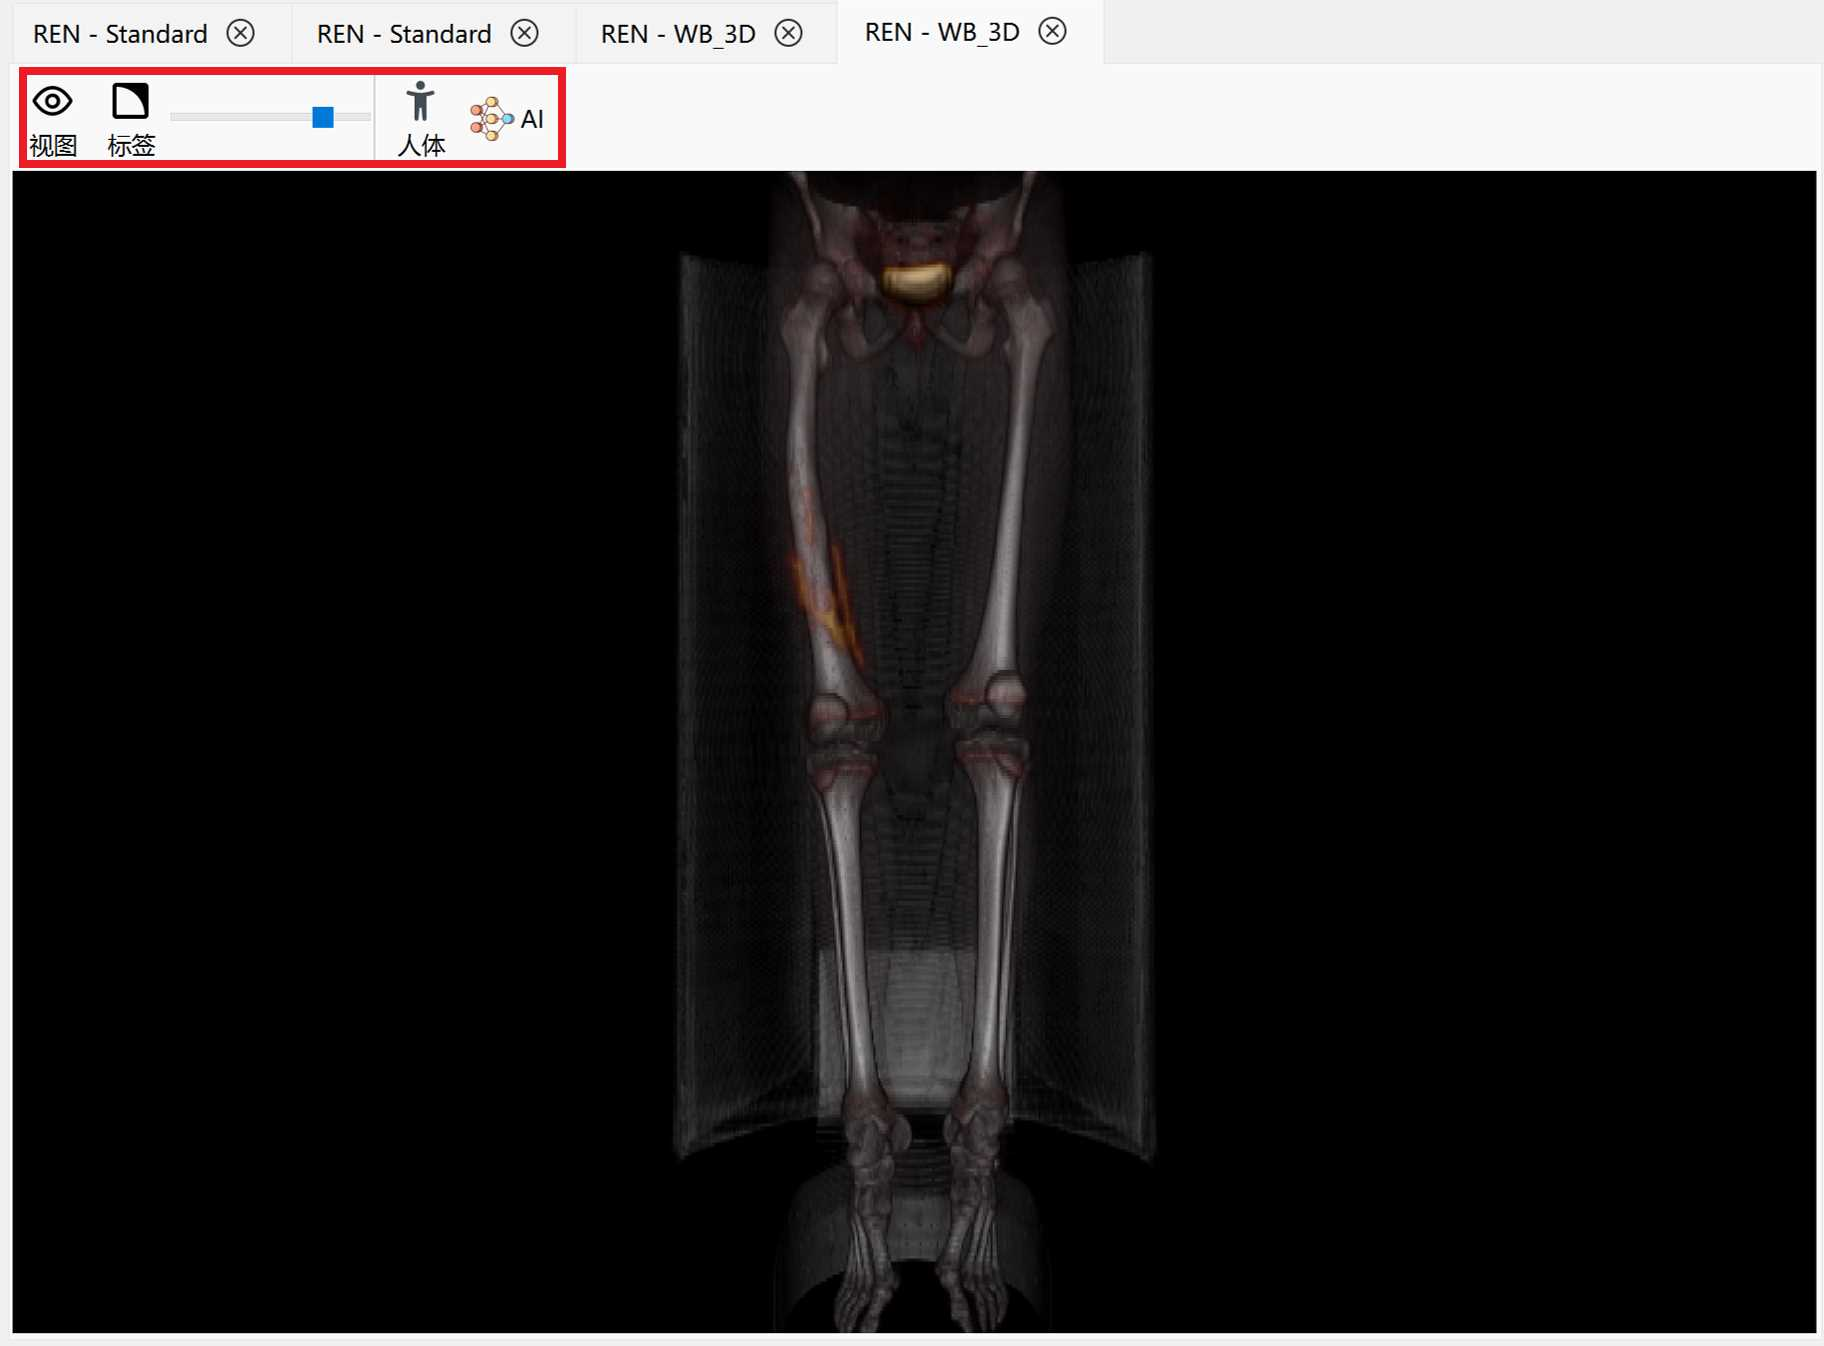
\includegraphics[width=0.49\linewidth]{figures/chap05_view_3DF.jpg}
    \label{fig:chap05_view_3DF}
  }
  \newline
  \caption{可视化区域示意图}\label{fig:chap05_view}
\end{figure}

在影像的二维可视化中,工具栏前端不仅显示了当前视图信息,同时展示了位于可视化区域中心蓝色十字准星所指示的像素位置坐标及其相关的影像值,这些信息用于评估和分析至关重要。值得说明的是,坐标可以进行修改,可视化区域也会随之进行更新。工具栏包含了多种功能按钮:视图按钮用于变换不同的视角;操作按钮允许用户复原图像、执行旋转及进行镜像翻转;鼠标左键图标按钮则使用户能够通过鼠标左键拖拽影像或移动蓝色虚线十字准星;切换按钮则可以让鼠标滑轮的功能在切换切片和缩放之间进行转换;对比度按钮则用以调整可视化影像的对比度。此外,还包含了导入分割图像或者边界框的标签按钮,调节标签透明度的滑块,以及用于给出辅助诊断建议的AI按钮。

在影像的三维可视化工具栏中,视图功能按钮使用户能够选择展示整体影像数据或仅展示根据标签图导入的边界框所分割的部分;标签功能按钮方便用户导入标注病灶区域的边界框;透明度调节滑块通过精细控制,使得边界框标签透明度得以调整;而人体功能按钮则在PET/CT影像融合展示中,提供了移除机床视图的选项;同样地,AI按钮针对三维影像提供辅助诊断功能。此外,用户可通过鼠标左键操控,使影像围绕其几何中心在三维空间内进行旋转,而鼠标滚轮则赋予了以影像中心作为锚点进行放大或缩小的功能。

\section{自动诊断}


自动诊断方法,作为本章研究中辅助诊断模块的核心组成部分,集成了基于\(^{99m}\)Tc-MDP动态骨显像的假体关节感染辅助诊断框和基于\(^{18}\)F-FDG PET/CT三维影像的下肢骨折相关感染检测与诊断框架。在用户界面上,该集成的自动诊断方法通过一个简洁的AI按钮呈现于标签页的顶部工具栏中,从而在可视化显示区域中直观地提供使用接入点。

\subsection{辅助诊断模块}

通过简单地点击AI按钮,辅助诊断模块便可迅速触发内嵌的深度学习算法,进而自动对当前可视化的医学影像进行分析。特别地,辅助诊断模块会从医学影像的元数据中自动提取关键信息,以确保算法的适用性。算法开始对影像数据进行深入分析时,将对病灶区域进行精准的辅助诊断,并以直观的方式展现出来。

\begin{figure}[htbp]
  \centering
  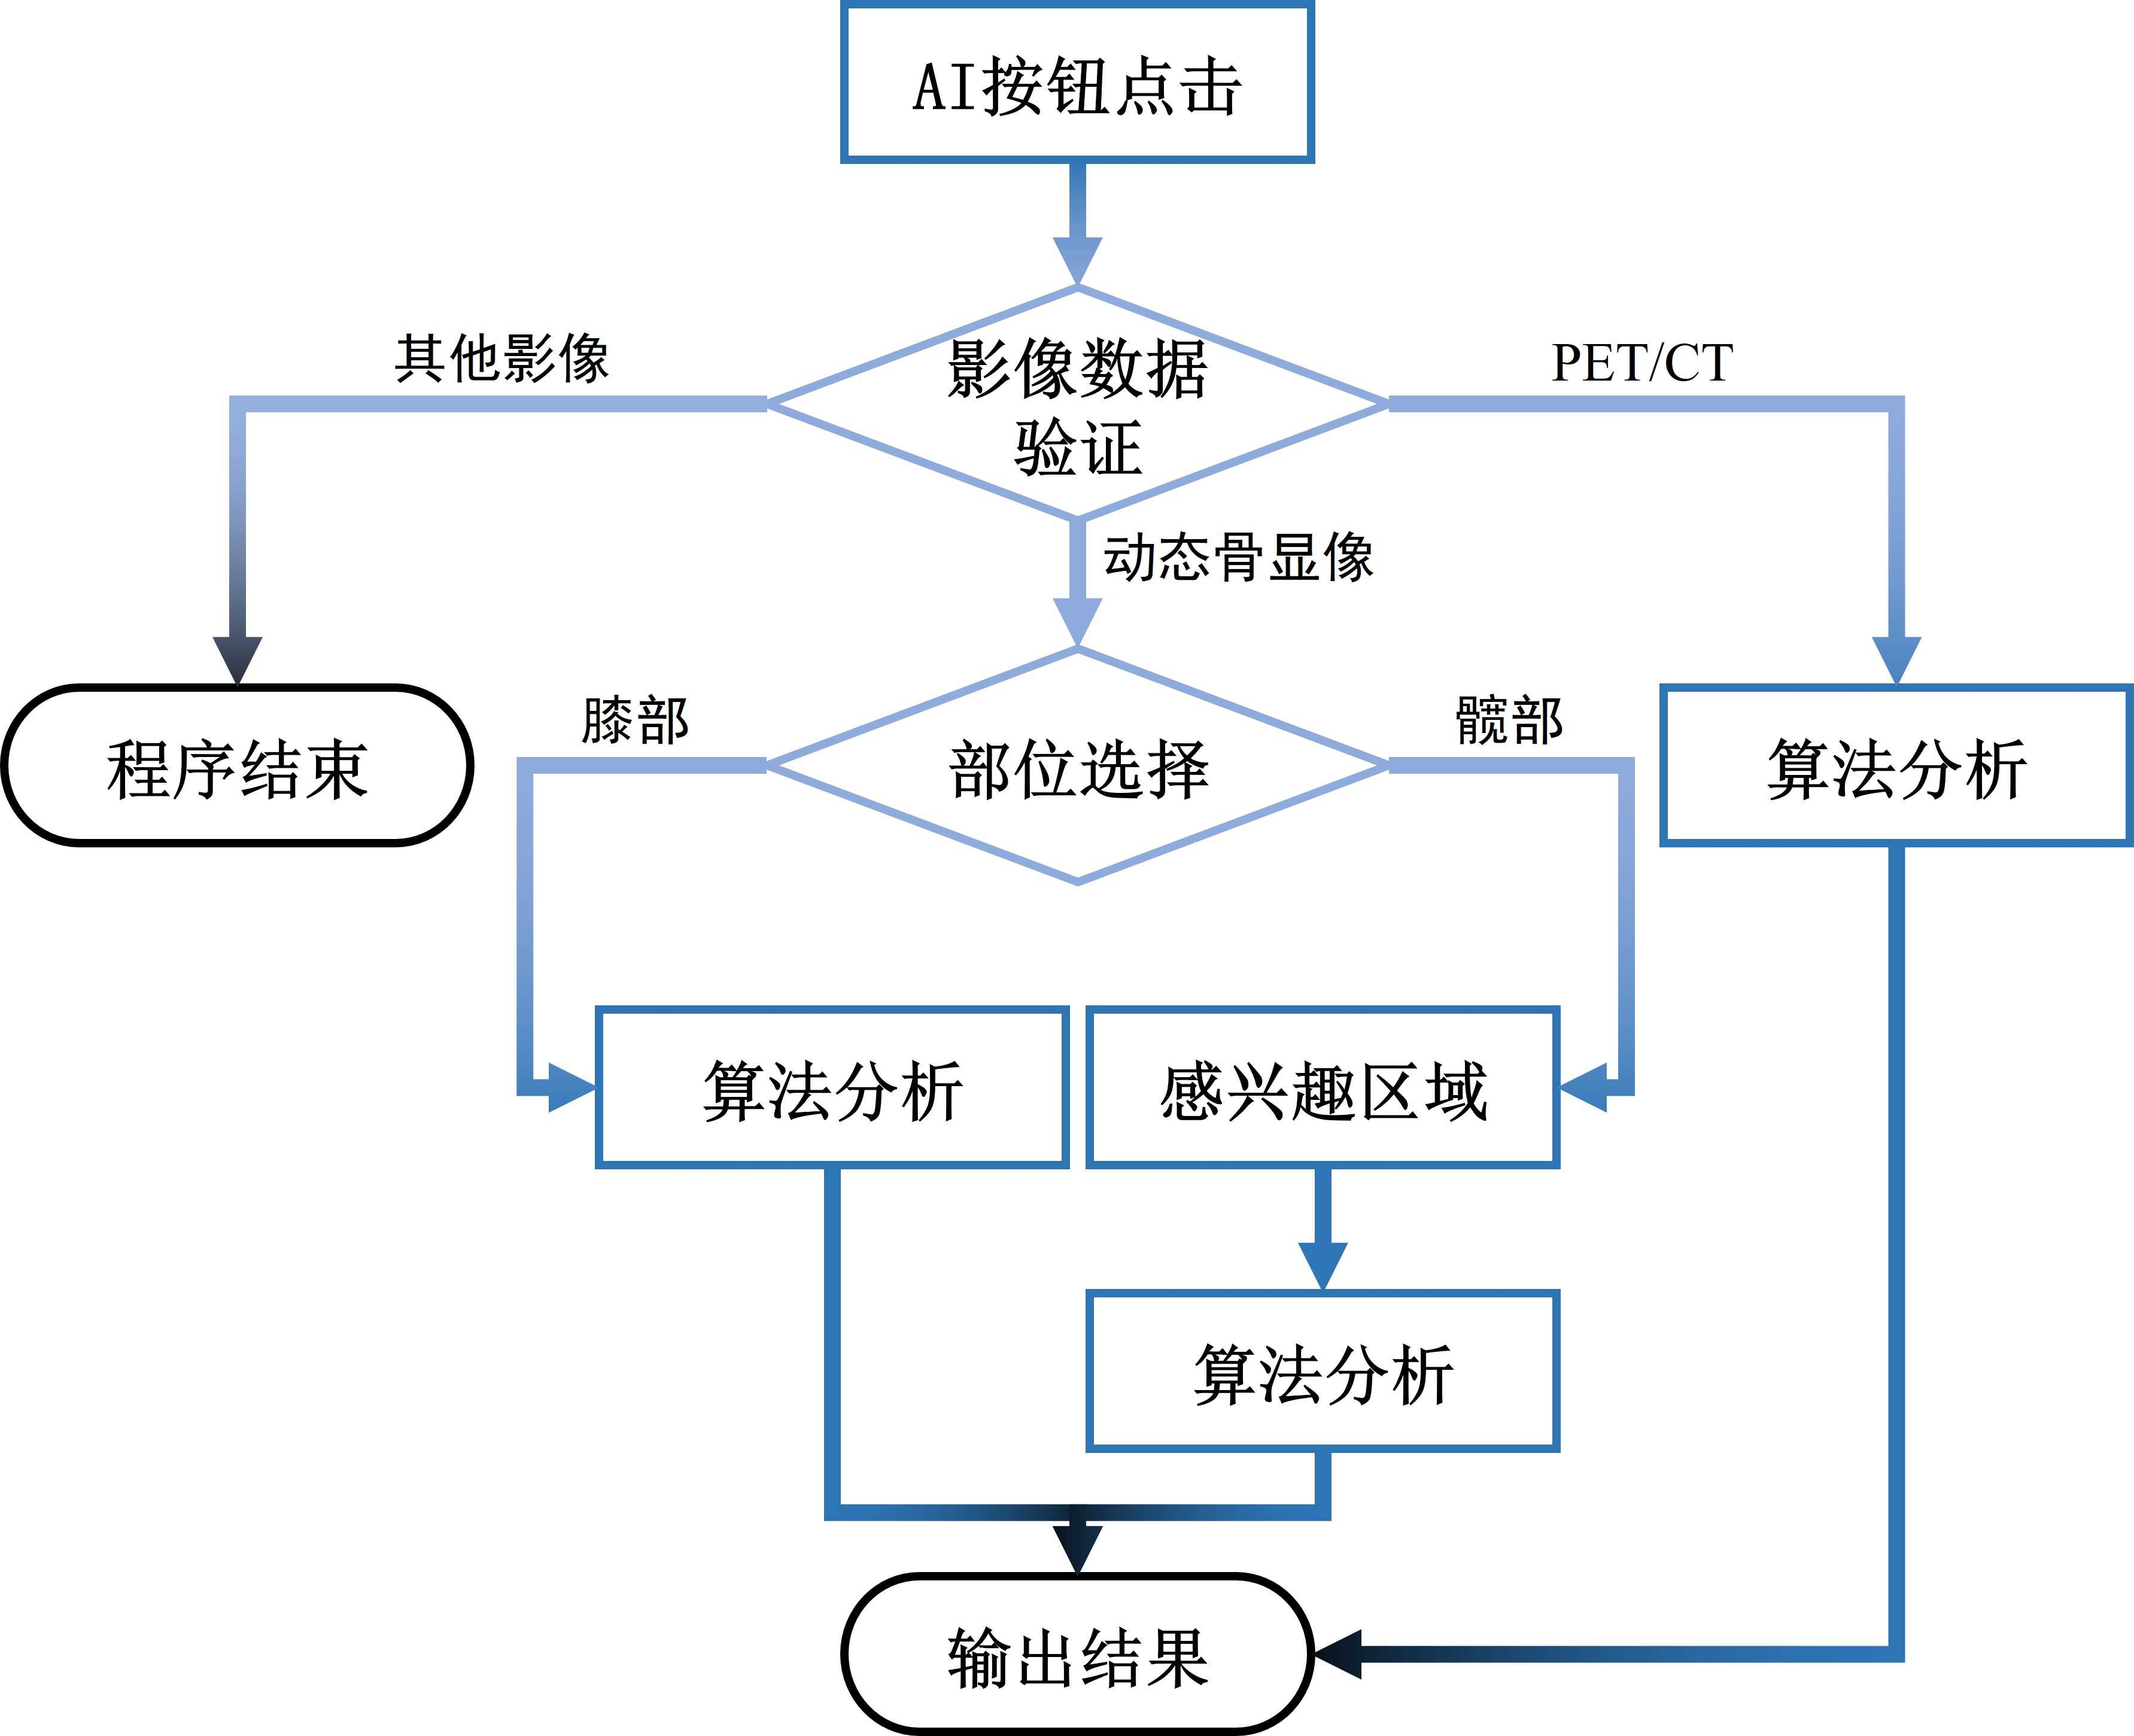
\includegraphics[width=0.9\textwidth]{figures/chap05_diagnose.jpg}
  \caption{辅助诊断模块的整体运行流程}
  \label{fig:chap05_diagnose}
\end{figure}

图\ref{fig:chap05_diagnose}展示了辅助诊断模块的整体运行流程。在初始阶段,对医学影像的元数据进行解析,从而识别所可视化的影像的模态。当遇到不兼容的影像模态时,辅助诊断模块会通过信息框提示用户,流程于此终止。

若影像模态确认为动态骨显像时,则会引导用户在膝部和髋部之间进行选择。选定膝部后,辅助诊断模块会立即采用第三章的框架,执行病灶的辅助诊断,同时通过计时弹窗提示程序正在运行中以及运行时间。髋部选择路径稍有不同,流程会进入一个选择感兴趣区域的环节。用户通过鼠标左键按下生成一个\(40 \times 40\)的红色边框,并在可视化区域中移动到理想的区域。随后,释放鼠标左键,辅助诊断模块将以鼠标位置为中心的\(40 \times40 \)的区域设置为感兴趣区域并提供给第三章的框架用于进一步分析和诊断。

若影像模态确认为PET/CT时,辅助诊断模块会自主调用第四章的检测诊断框架,开始识别和评估潜在的病变区域,同时通过计时弹窗提示用户。在算法运行结束后,辅助诊断结果不仅以弹窗的形式对用户进行提示,同时在PET/CT中绘制出特定的边界框标注,从而实现了一个高效、直观且用户交互性强的辅助诊断工作流。

\section{可视化}

在本章研究中,可视化方法发挥着至关重要的作用,其由文件解析、可视化以及影像分析三大关键功能模块构成。文件解析模块构成了可视化方法的基石,它的主要职责在于解析影像文件数据,并将其重塑为三维医学影像,为之后的展示与分析奠定重要基础。可视化模块则构成了可视化方法的核心,该模块负责将解析后的医学影像数据转化并映射至自然图像领域中常规应用的色彩空间,其目的是提高影像的可读性的同时,使得医学影像的关键信息在视觉上更加明显。最后,影像分析模块代表了可视化方法的进阶扩展,它操控着对视觉呈现的医学影像的进一步图像处理,如调整对比度和缩放等。此模块便于用户进行细节分析,包括识别和解读影像上的关键特征,从而全面地挖掘影像所蕴含的深层次信息。

\subsection{文件解析模块}

在初始阶段,文件解析模块会将医学影像中原始的像素值转换为更适合用于评估和分析的影像值,用以确保了影像信息的临床相关性,还为后续的量化分析提供了定量的指标。例如,CT影像中原始像素值被转换成HU,PET影像的原始像素值则被转换为SUV。

对于DICOM文件,解析过程如下:
\begin{enumerate}[1)]
  \item 读取需解析的DICOM文件所在路径下的所有DICOM文件。
  \item 根据元数据中的Study Instance UID将这些文件划分到不同的研究组中。
  \item 根据元数据中的Series Instance UID进一步在研究组中划分为不同的系列组。
  \item 根据每个文件的影像大小,在系列组中再进一步划分为不同的尺寸组。
  \item 根据元数据中的Slice Location或Instance Number对尺寸组中的文件进行排序。
  \item 依次将每个尺寸组的文件组成一个完整的医学影像,并转换像素值为影像值。
  \item 数据以研究组、系列组、尺寸组和医学影像为顺序的层次化结构进行展示。
\end{enumerate}

在NIfTI(Neuroimaging Informatics Technology Initiative)文件的解析过程中,由于这类文件并不包含像DICOM格式那样丰富的元数据,因此其解析过程相对简单。解析一开始是读入NIfTI文件,并为之分配随机生成的Study Instance UID与Series Instance UID。接着读取该文件中的影像数据并获取影像大小。最终解析后的数据将按照一种与DICOM相同的层次化结构进行呈现。

\subsection{可视化模块}

在文件解析结束之后,可视化模块将对不同模态的医学影像数据采取差异化的可视化处理策略,具体可分为二维和三维两个维度,各自又包含单一模态展示和双模态融合展示两种处理方法。

对于二维展示,为了将医学影像值有效地映射到自然图像领域中的RGB色彩空间,可视化模块采用了最大最小值归一化方法,确保医学影像值可以在保持其诊断信息的同时,以一种标准化且用户直观理解的视觉形式进行展现。其计算方式如下:
\begin{equation}
  v =\text{floor}(\frac{v - \min(v)}{\max(v) - \min(v)} \times 255)
  \label{eq:chap05_min_max}
\end{equation}
其中,\(\text{floor}(\cdot)\)表示向下取整函数,\(\max(\cdot)\)表示计算最大值的函数,\(\min(\cdot)\)表示计算最小值的函数。

颜色映射是用于将数据值映射到颜色的一种方法,可以使数据分布、趋势和特征以更加直观的方式得以呈现。图\ref{fig:chap05_colormap}展示了三种颜色映射:binary是一种简单的黑白二色的颜色映射,其中较小的值映对应黑色而较大的值对应白色;gray颜色映射通过灰阶色调展示图像或数据的亮度等级;hot是一种常用于表示温度或热度的颜色映射,整体上从黑色渐变到红色、黄色最终达到白色。这些颜色映射各具特色,能有效地增强数据的视觉效果和解读性。

\begin{figure}[htbp]
  \centering
  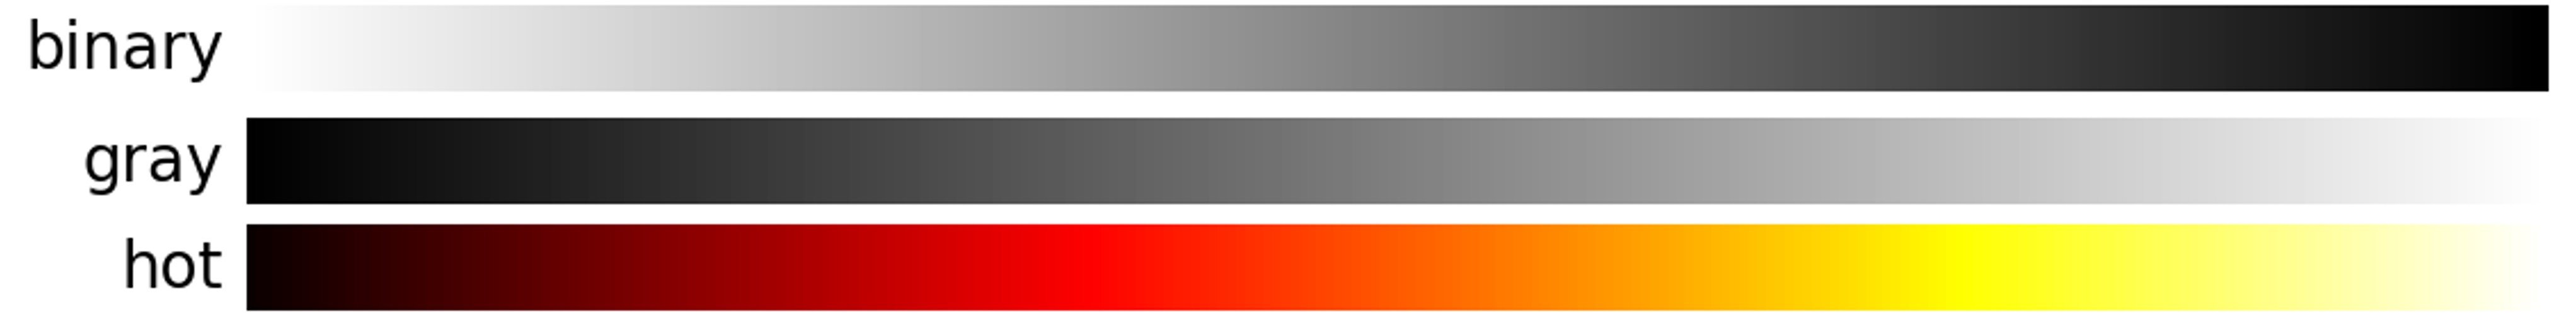
\includegraphics[width=\textwidth]{figures/chap05_colormap.jpg}
  \caption{三种不同的颜色映射}
  \label{fig:chap05_colormap}
\end{figure}

接下来,不同模态的影像值将采用不同的颜色映射,以增强影像中各区域之间的对比度和其可视性效果,如算法\ref{algo:chap05_colormap}所示。

\begin{algorithm}
  \caption{医学影像着色处理}
  \label{algo:chap05_colormap}
  \SetKwInOut{Input}{输入}
  \SetKwInOut{Output}{输出}
  \Input{医学影像$\mathcal{I}$}
  \Output{颜色映射$cm$}
  \vspace{5pt}

  \lIf(\tcp*[f]{无需进行着色处理}){$\mathcal{I} = \text{RGB}$}{$cm \leftarrow \text{None}$}
  \lElseIf(\tcp*[f]{gray体现不同解剖结构的层次}){$\mathcal{I} \in \{CT,MRI\}$}{$cm \leftarrow \text{gray}$}
  \uElseIf{$\mathcal{I} \in \{PET,NM\}$}{
    \lIf(\tcp*[f]{hot在融合时强调高摄取区域}){双模态融合可视化}{$cm \leftarrow \text{hot}$}
    \lElse(\tcp*[f]{单模态可视化}){$cm \leftarrow \text{binary}$}
  }
  \lElse{$cm \leftarrow \text{gray}$}
\end{algorithm}

在完成医学影像的颜色映射之后,重要的一步是考虑可视化区域的尺寸\((w,h)\)、三维医学影像在各个方向上的尺寸\((x,y,z)\)以及体素间距(Spacing\(=(s_x,s_y,s_z)\))。这一步骤是为了保证医学影像能够完整地填充整个可视化区域,以便用户能够得到一个清晰且准确的视图。因此,在进行三维医学影像切片的可视化处理时,需要计算相应的缩放比例,以便影像切片能够适配可视化区域。相关的缩放比例计算方式如下:
\begin{equation}
  \begin{aligned}
    \mathcal{S}_x^{h} & = s_y \times min(\frac{h}{z \times s_z}, \frac{w}{y \times s_y}) & \quad \mathcal{S}_x^{w} & = s_z \times min(\frac{h}{z \times s_z}, \frac{w}{y \times s_y}) \\
    \mathcal{S}_y^{h} & = s_x \times min(\frac{h}{z \times s_z}, \frac{w}{x \times s_x}) & \quad \mathcal{S}_y^{w} & = s_z \times min(\frac{h}{z \times s_z}, \frac{w}{x \times s_x}) \\
    \mathcal{S}_z^{h} & = s_x \times min(\frac{h}{x \times s_x}, \frac{w}{y \times s_y}) & \quad \mathcal{S}_z^{w} & = s_y \times min(\frac{h}{x \times s_x}, \frac{w}{y \times s_y}) \\
  \end{aligned}
  \label{eq:chap05_scale}
\end{equation}
其中,\(\mathcal{S}_\cdot^{h},\mathcal{S}_\cdot^{w}\)分别代表三维影像中,垂直于\(\cdot\)轴的切片在可视化过程中,所需应用在高度与宽度方向上的缩放比例。

最终,三维医学影像的对应切片将由可视化模块根据预设的坐标及视图参数来进行展现。当进行双模态影像的融合展示时,首先是在两种不同模态的影像之间采用第四章中介绍的方法进行配准。完成配准后,依据设定的坐标和视图参数,两种模态的影像切片将被融合展示。图像融合可以采用以下加权平均的计算方式:
\begin{equation}
  \text{Image} = \alpha \times \text{Image}_1 + \beta \times \text{Image}_2
  \label{eq:chap05_fusion}
\end{equation}
其中,\(\text{Image}_1,\text{Image}_2\)分别代表了待融合的的两幅图像,而融合系数\(\alpha, \beta\),分别取值为0.3和0.7,用以控制融合过程中各图像的权重。

对于三维展示,本章提出的方法采用了Visualization Toolkit(VTK)库来实现医学影像的三维可视化处理。首先,将医学影像数据包含的三维矩阵和体素间距以及自定义的影像原点导入到VTK中,并转换成适合VTK处理的图像格式。为了确保生成的三维影像中心位于坐标原点\((0,0,0)\),将医学影像的原点设定为:
\begin{equation}
  \begin{aligned}
    o_x & = -0.5 \times size_x \times spacing_x \\
    o_y & = -0.5 \times size_y \times spacing_y \\
    o_z & = -0.5 \times size_z \times spacing_z \\
  \end{aligned}
\end{equation}
其中,\(o_x,o_y,o_z\)分别代表医学影像在三维空间中的原点坐标,\(size_x,size_y,size_z\)分别代表医学影像在各轴方向上的大小,\(spacing_x,spacing_y,spacing_z\)则为各轴方向上的体素间距。

随后,可视化模块使用了VTK中一种基于光线投射的体渲染技术,该技术通过射出光线,对体数据进行采样与体素插值,从而生成包含了透明度、颜色以及光照效果的三维影像,创造出具有立体感的体渲染图,如图\ref{fig:chap05_view_3D}所示。

考虑到该体渲染技术的特性,可视化模块设定了将医学影像的影像值转换为相应颜色以及透明度的映射表,并设置了必要的光照参数,包括环境光照、漫反射光照和镜面反射光照的强度。在三维模型构建完成后,通过调整观察相机的位置和方向,可以生成完整详尽的三维视图,以供医疗专家进行深入分析和解读。具体而言,为展示完整的三维医学影像,相机的视角设定为60°,焦点设置在\((0,0,0)\),朝上方向设置为\((0,0,1)\),位置定位在\((0,P_y,0)\)。其中\(P_y\)的计算方式如下:
\begin{equation}
  P_y = -0.5 \times \max(size_x \times spacing_x, size_z \times spacing_z) \div \tanh(\pi / 6)\\
\end{equation}

在双模态融合展示方面,可视化模块依据以上方法,分别对两种不同模态的医学影像进行独立的三维渲染并直接进行展示,如图\ref{fig:chap05_view_3DF}所示。

\subsection{影像分析模块}

在完成可视化模块的处理后,影像分析模块会给二维和三维展示的医学影像提供各种功能。如图\ref{fig:chap05_view_2D}和\ref{fig:chap05_view_2DF}所示,在二维影像分析时,包含了全部功能的工具栏位于标签页顶部。包含视图、坐标和对应影像值的信息区域与可视化区域内的影像切片及蓝色十字标记相互联动,任何一处发生变动,其他位置也会随之更新。主要的映射关系包括:
\begin{enumerate}
  \item \(\text{鼠标位置} \rightarrow \text{场景位置} \rightarrow \text{图像坐标}\)\label{en:chap05_1}。
  \item \(\text{图像坐标} \rightarrow \text{场景位置}\)\label{en:chap05_2}。
\end{enumerate}

坐标信息可以直接被修改,依据映射关系\ref{en:chap05_2}更新蓝色十字的位置及相应切片。使用鼠标左键可移动蓝色十字,并依照映射关系\ref{en:chap05_1}刷新坐标和影像值信息。视图信息可以通过按键切换不同视图下的影像切片,并根据当前坐标信息来更新蓝色十字的指向位置。鼠标滚轮则通过调整当前的坐标信息来更新影像切片和蓝色十字的位置。操作按钮提供了实施旋转、镜像翻转以及图像重置的仿射变换功能。普通按钮允许用户修改鼠标左键的操作,以实施影像的平移变换,而切换按钮则改变鼠标滚轮的作用,从而实现影像的缩放变换。所有这些操作均通过应用仿射变换矩阵来完成。二维仿射变换矩阵如下所示:
\begin{equation}
  \left[
    \begin{array}{ccc}
      a & b & t_x \\
      c & d & t_y \\
      0 & 0 & 1   \\
    \end{array}
    \right]
  \label{eq:chap05_affine_mat}
\end{equation}
其中,\(a\)和\(d\)表示缩放因子,\(b\)和\(c\)用于旋转变换之中,\(t_x\)和\(t_y\)表示平移量。通过调整这些参数,可以实现不同的仿射变换,如下所示:
\begin{equation}
  \begin{array}{ccc}
    \text{旋转} & \text{缩放} & \text{镜像} \\
    \left[
      \begin{array}{ccc}
        \cos(\theta) & -\sin(\theta) & 0 \\
        \sin(\theta) & \cos(\theta)  & 0 \\
        0            & 0             & 1 \\
      \end{array}
    \right]     &
    \left[
      \begin{array}{ccc}
        s_x & 0   & 0 \\
        0   & s_y & 0 \\
        0   & 0   & 1 \\
      \end{array}
    \right]     &
    \left[
      \begin{array}{ccc}
        -1 & 0 & 0 \\
        0  & 1 & 0 \\
        0  & 0 & 1 \\
      \end{array}
      \right] \quad
    \left[
      \begin{array}{ccc}
        1 & 0  & 0 \\
        0 & -1 & 0 \\
        0 & 0  & 1 \\
      \end{array}
    \right]                                 \\
  \end{array}
  \label{eq:chap05_affine}
\end{equation}
通过对比度按钮可以调节视图中医学影像的对比度,这是通过在弹出的窗口中输入窗位\(w_c\)和窗框\(w_w\),或者最大值\(ma\)和最小值\(mi\)来实现的。具体而言,对医学影像值\(v\)的计算如下所示:
\begin{equation}
  \begin{aligned}
    ma & = w_c + 0.5 \times w_w                       \\
    mi & = w_c - 0.5 \times w_w                       \\
    v  & = \frac{\min(\max(mi, v), ma) - mi}{ma - mi} \\
  \end{aligned}
  \label{eq:chap05_constrast}
\end{equation}
标签按钮可用来导入NIfTI格式的标签数据,以渲染分割图或显示边界框;标签滑块则可调整标签图的透明度。

在三维影像分析时,所有功能均汇聚于标签页顶部的工具栏中,如图\ref{fig:chap05_view_3D}和\ref{fig:chap05_view_3DF}所示。视图按钮允许用户选择性地渲染特定的影像数据,以此进行独立的视图展示。标签按钮用于导入NIfTI或Json格式的标签数据,这使得用户能够渲染出三维的立体边界框和关联分类标签。通过标签滑块,用户可细致地调整标签图层的透明度,以便更好地视察底层的医学影像。人体按钮采用了第四章中介绍的人体保留算法,专门针对PET/CT影像数据进行优化处理,去除掉机床等无关区域。此外,鼠标左键的操作,实现了观察摄像头在以原点为中心的虚拟球面的移动,来达成三维医学影像的旋转变换。同时,通过鼠标滑轮调节,可以改变三维影像与观察摄像头之间的距离,从而实现三维影像的缩放效果。

\section{案例分析}

在本节中,将示范自动诊断与可视化方法对上海市第六人民医院核医学科2016年的三个病例的应用实践:

(1)患者A在膝关节置换手术后两月接受了膝部的动态骨显像扫描,医生通过影像分析初步判定膝假体处可能感染,并在评估病症、临床表现以及影像与血液检验结果后,确诊为膝关节假体感染。

(2)患者B在髋关节置换术后两年进行了髋部动态骨显像扫描。经影像学分析后,医生怀疑髋假体发生感染,最终依据全面诊断确诊为假体髋关节感染。

(3)患者C在右股骨骨折治疗后接受PET/CT扫描。经过影像学判断,疑似存在感染性病灶。借助微生物培养、病理分析及临床综合判断,确认患有骨折相关感染。

\begin{figure}[htbp]
  \centering
  \subfloat[打开文件]{
    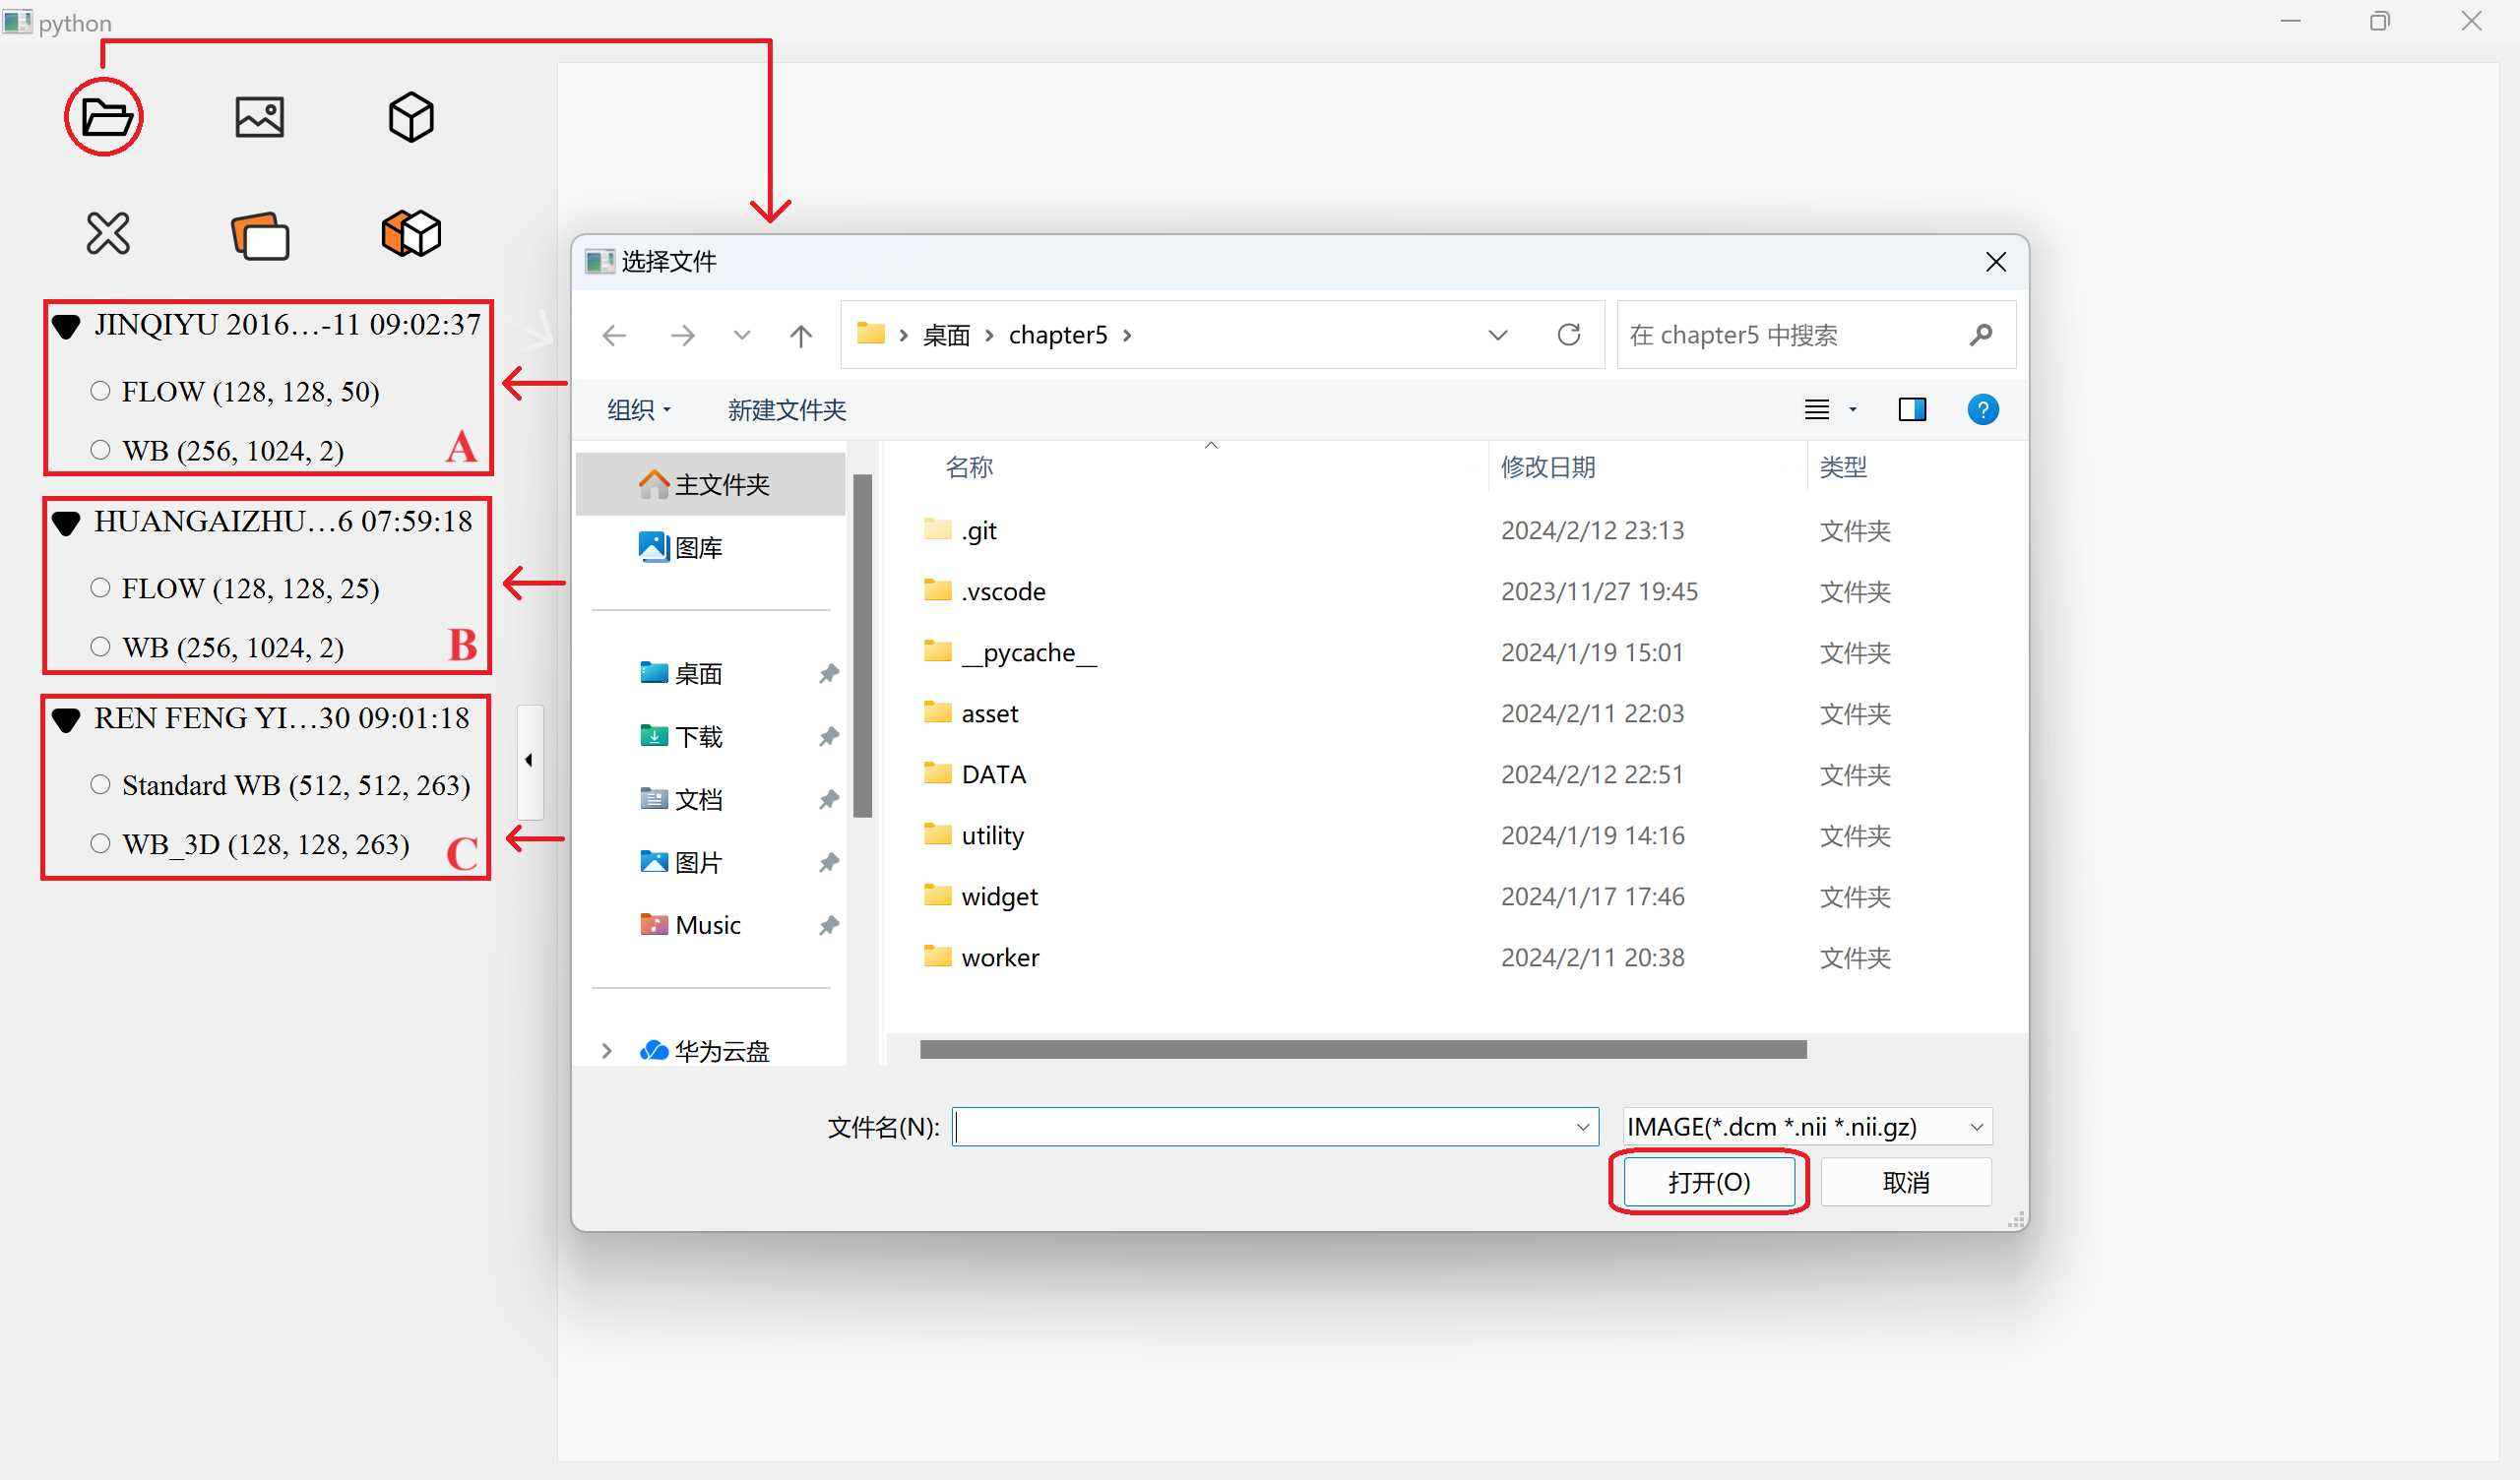
\includegraphics[width=0.49\textwidth]{figures/chap05_example01_open.jpg}
    \label{fig:chap05_example01_open}
  }
  \subfloat[膝部动态骨显像可视化]{
    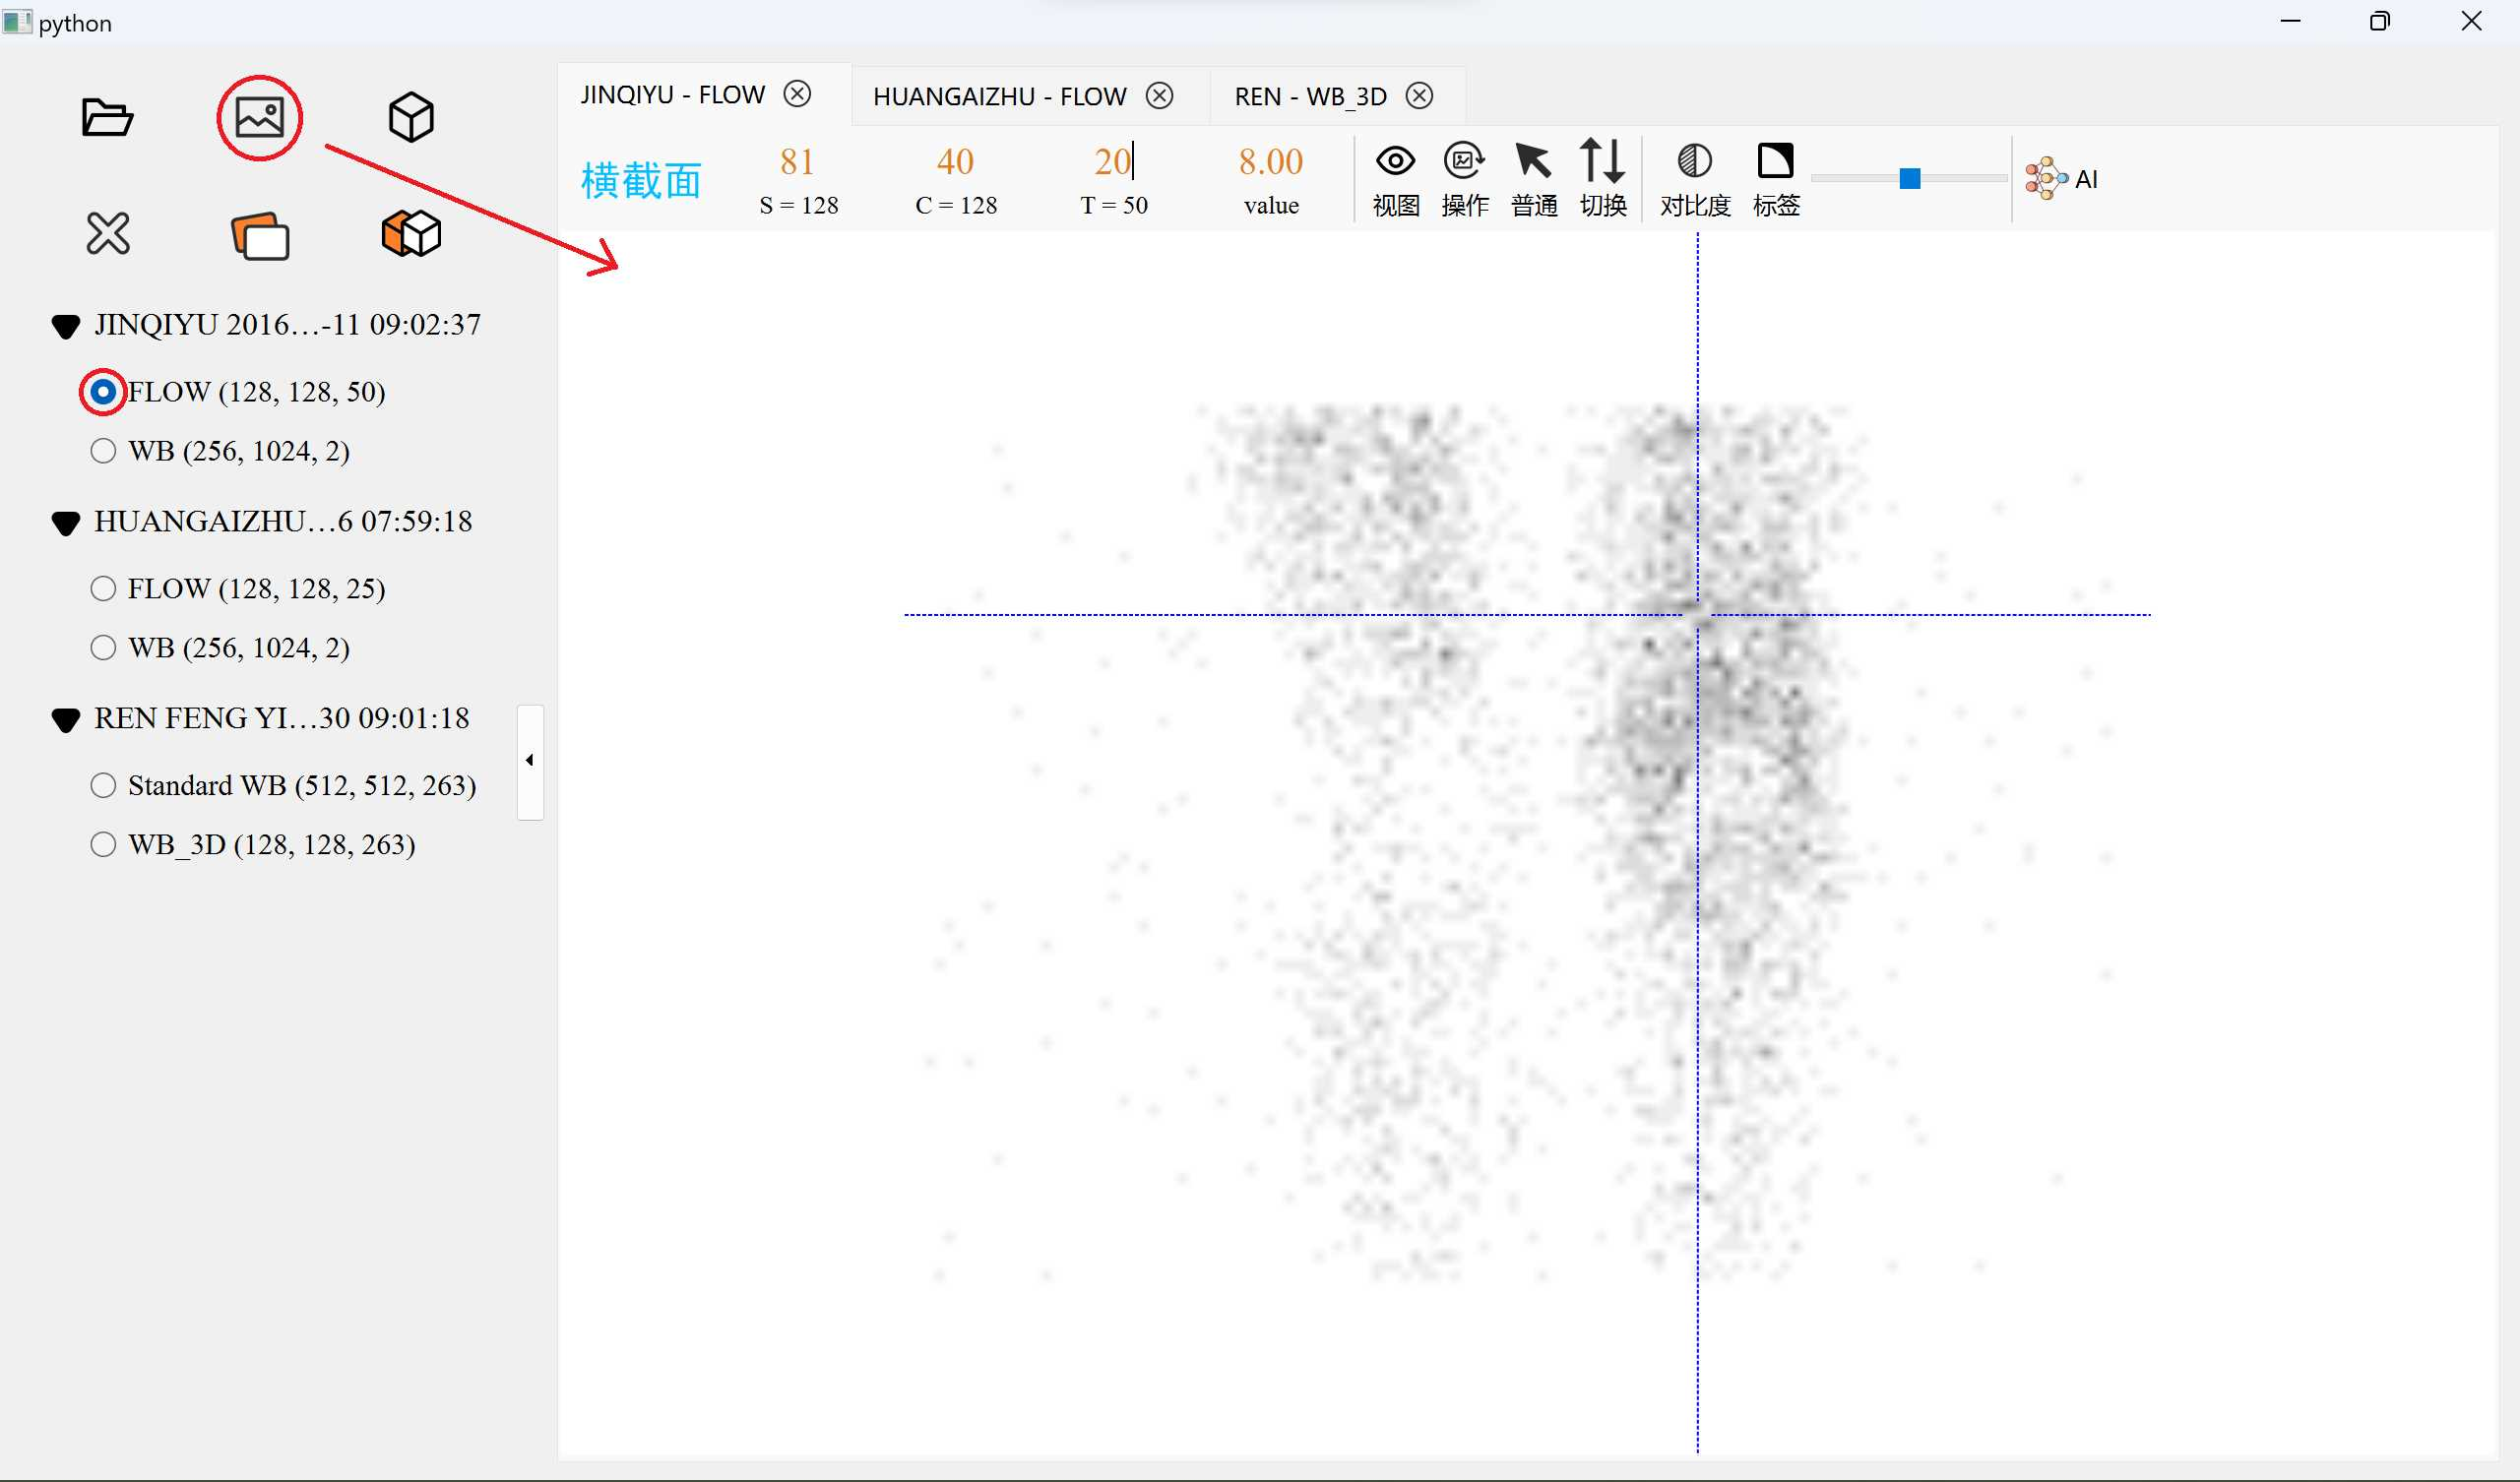
\includegraphics[width=0.49\textwidth]{figures/chap05_example02_vis.jpg}
    \label{fig:chap05_example02_vis}
  }
  \newline
  \newline
  \subfloat[髋部动态骨显像可视化]{
    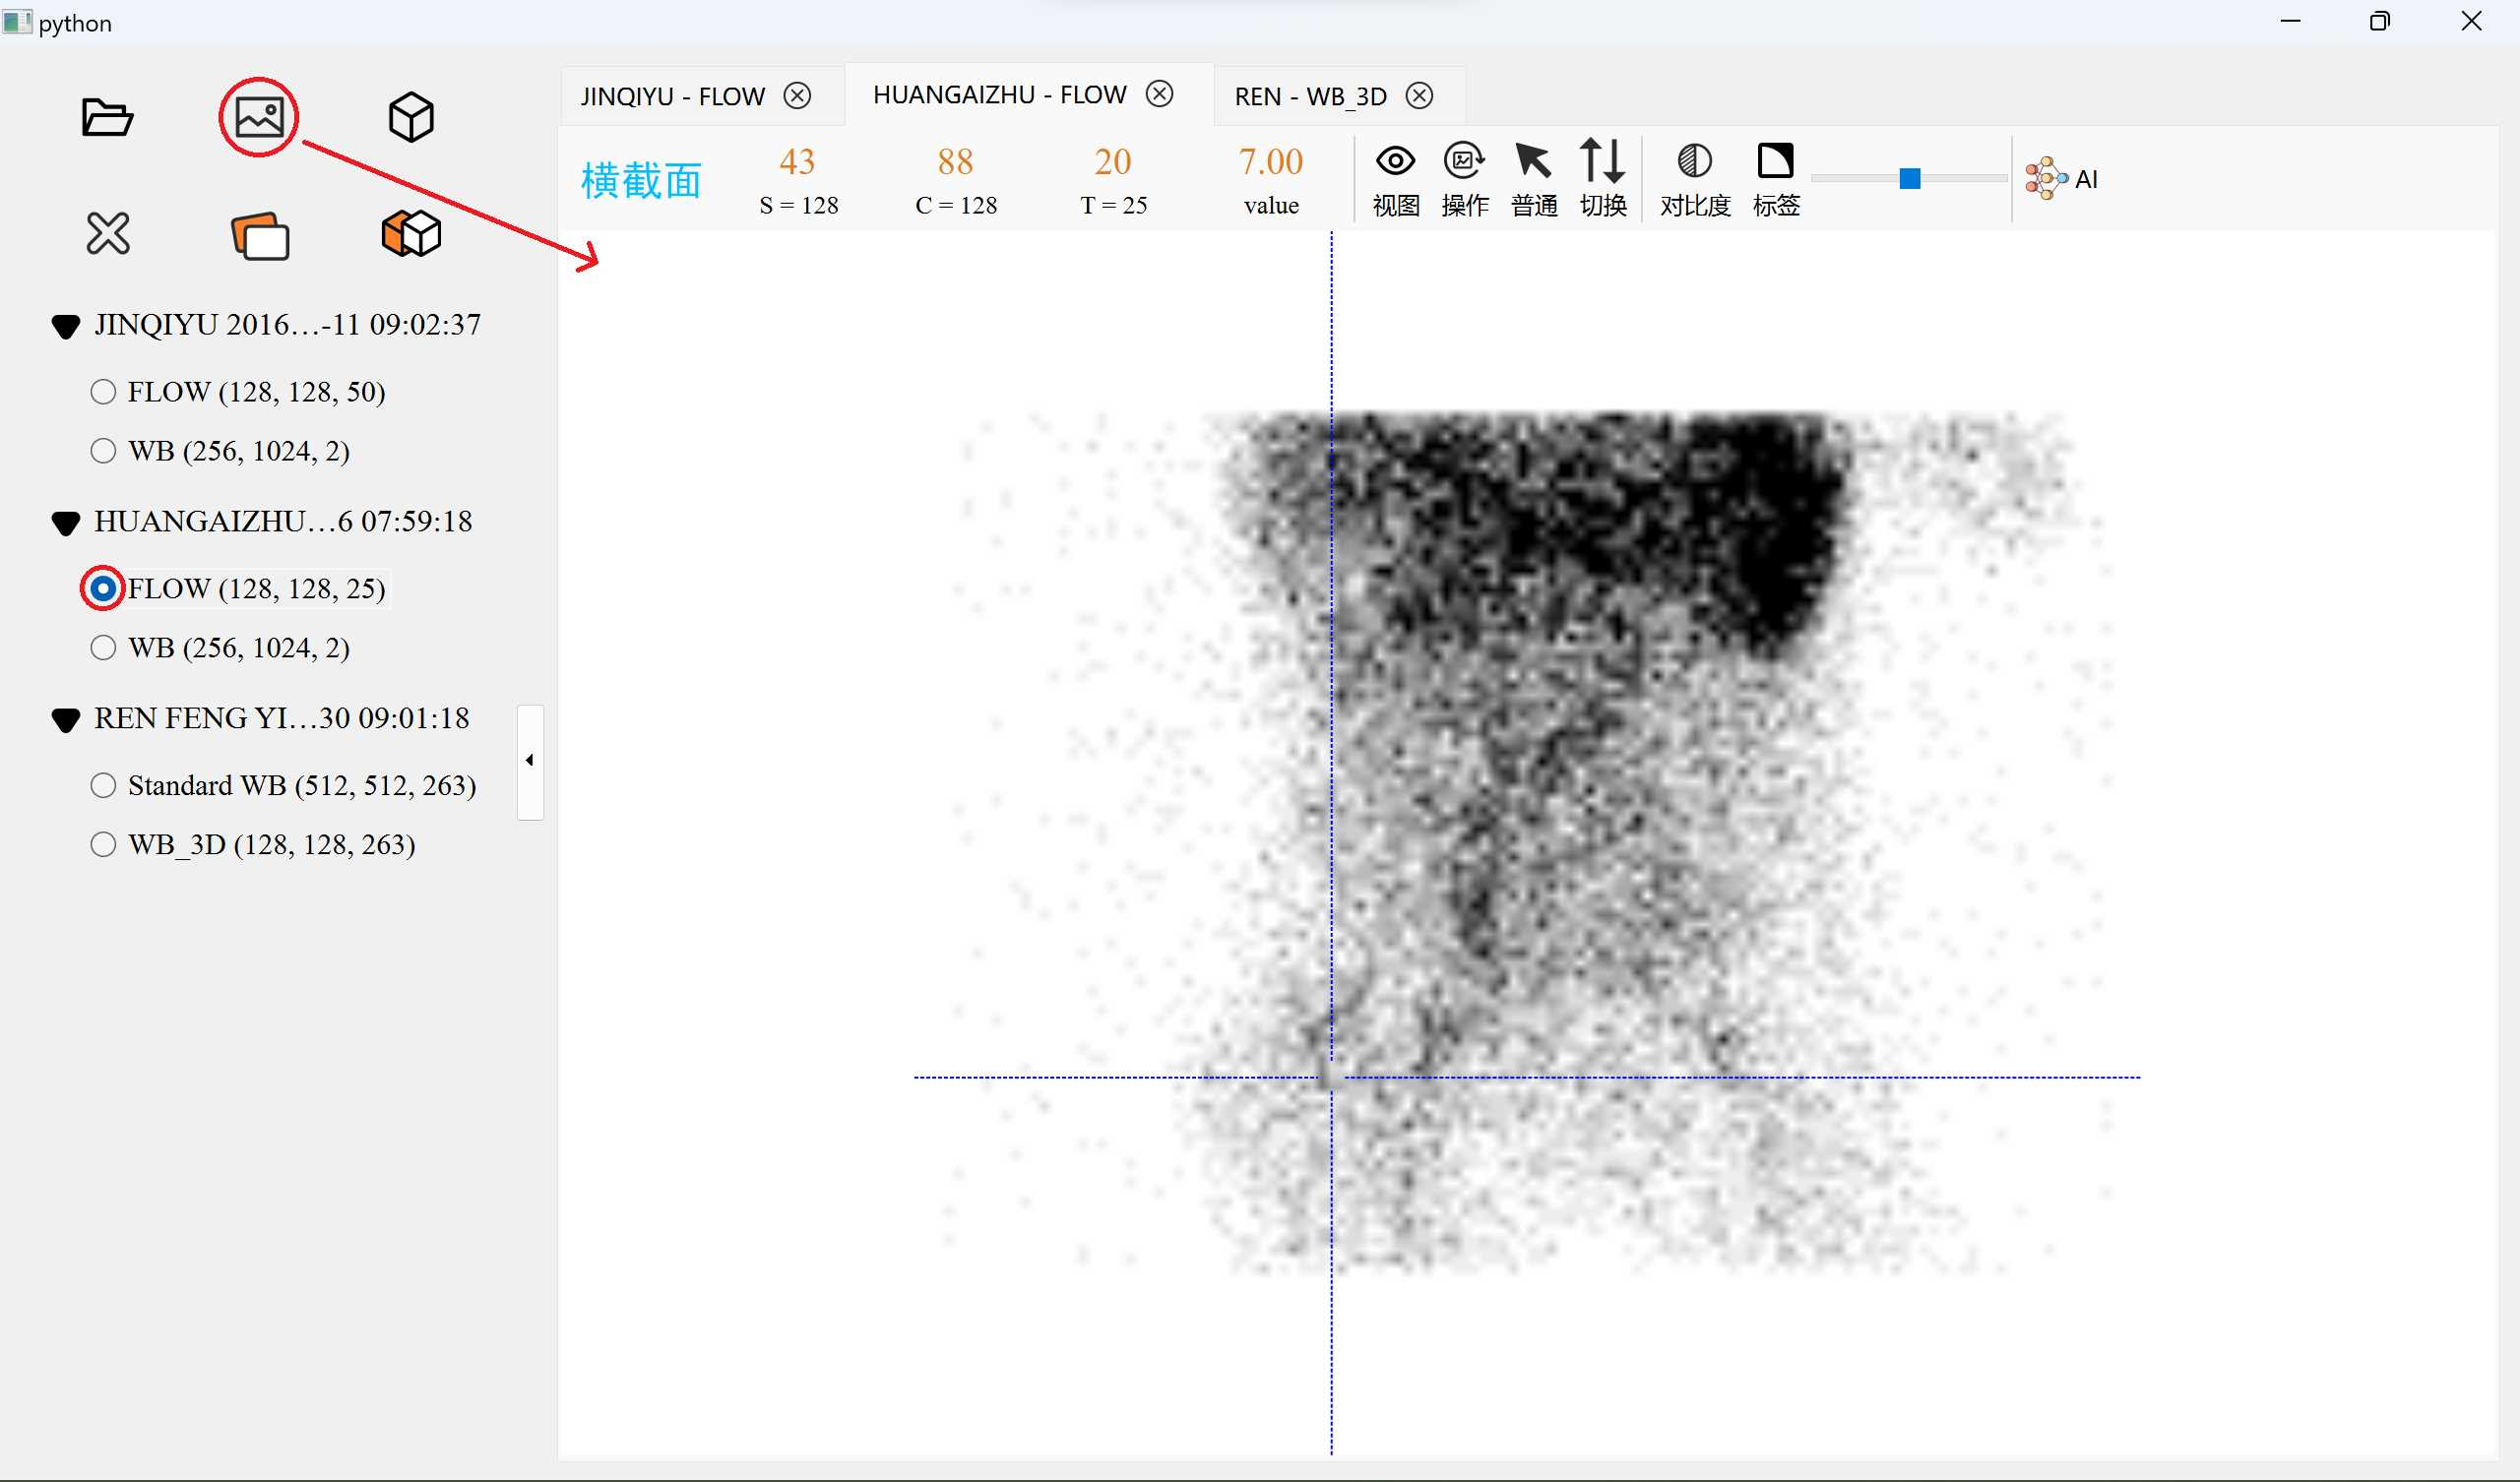
\includegraphics[width=0.49\textwidth]{figures/chap05_example03_vis.jpg}
    \label{fig:chap05_example03_vis}
  }
  \subfloat[下肢PET/CT融合可视化]{
    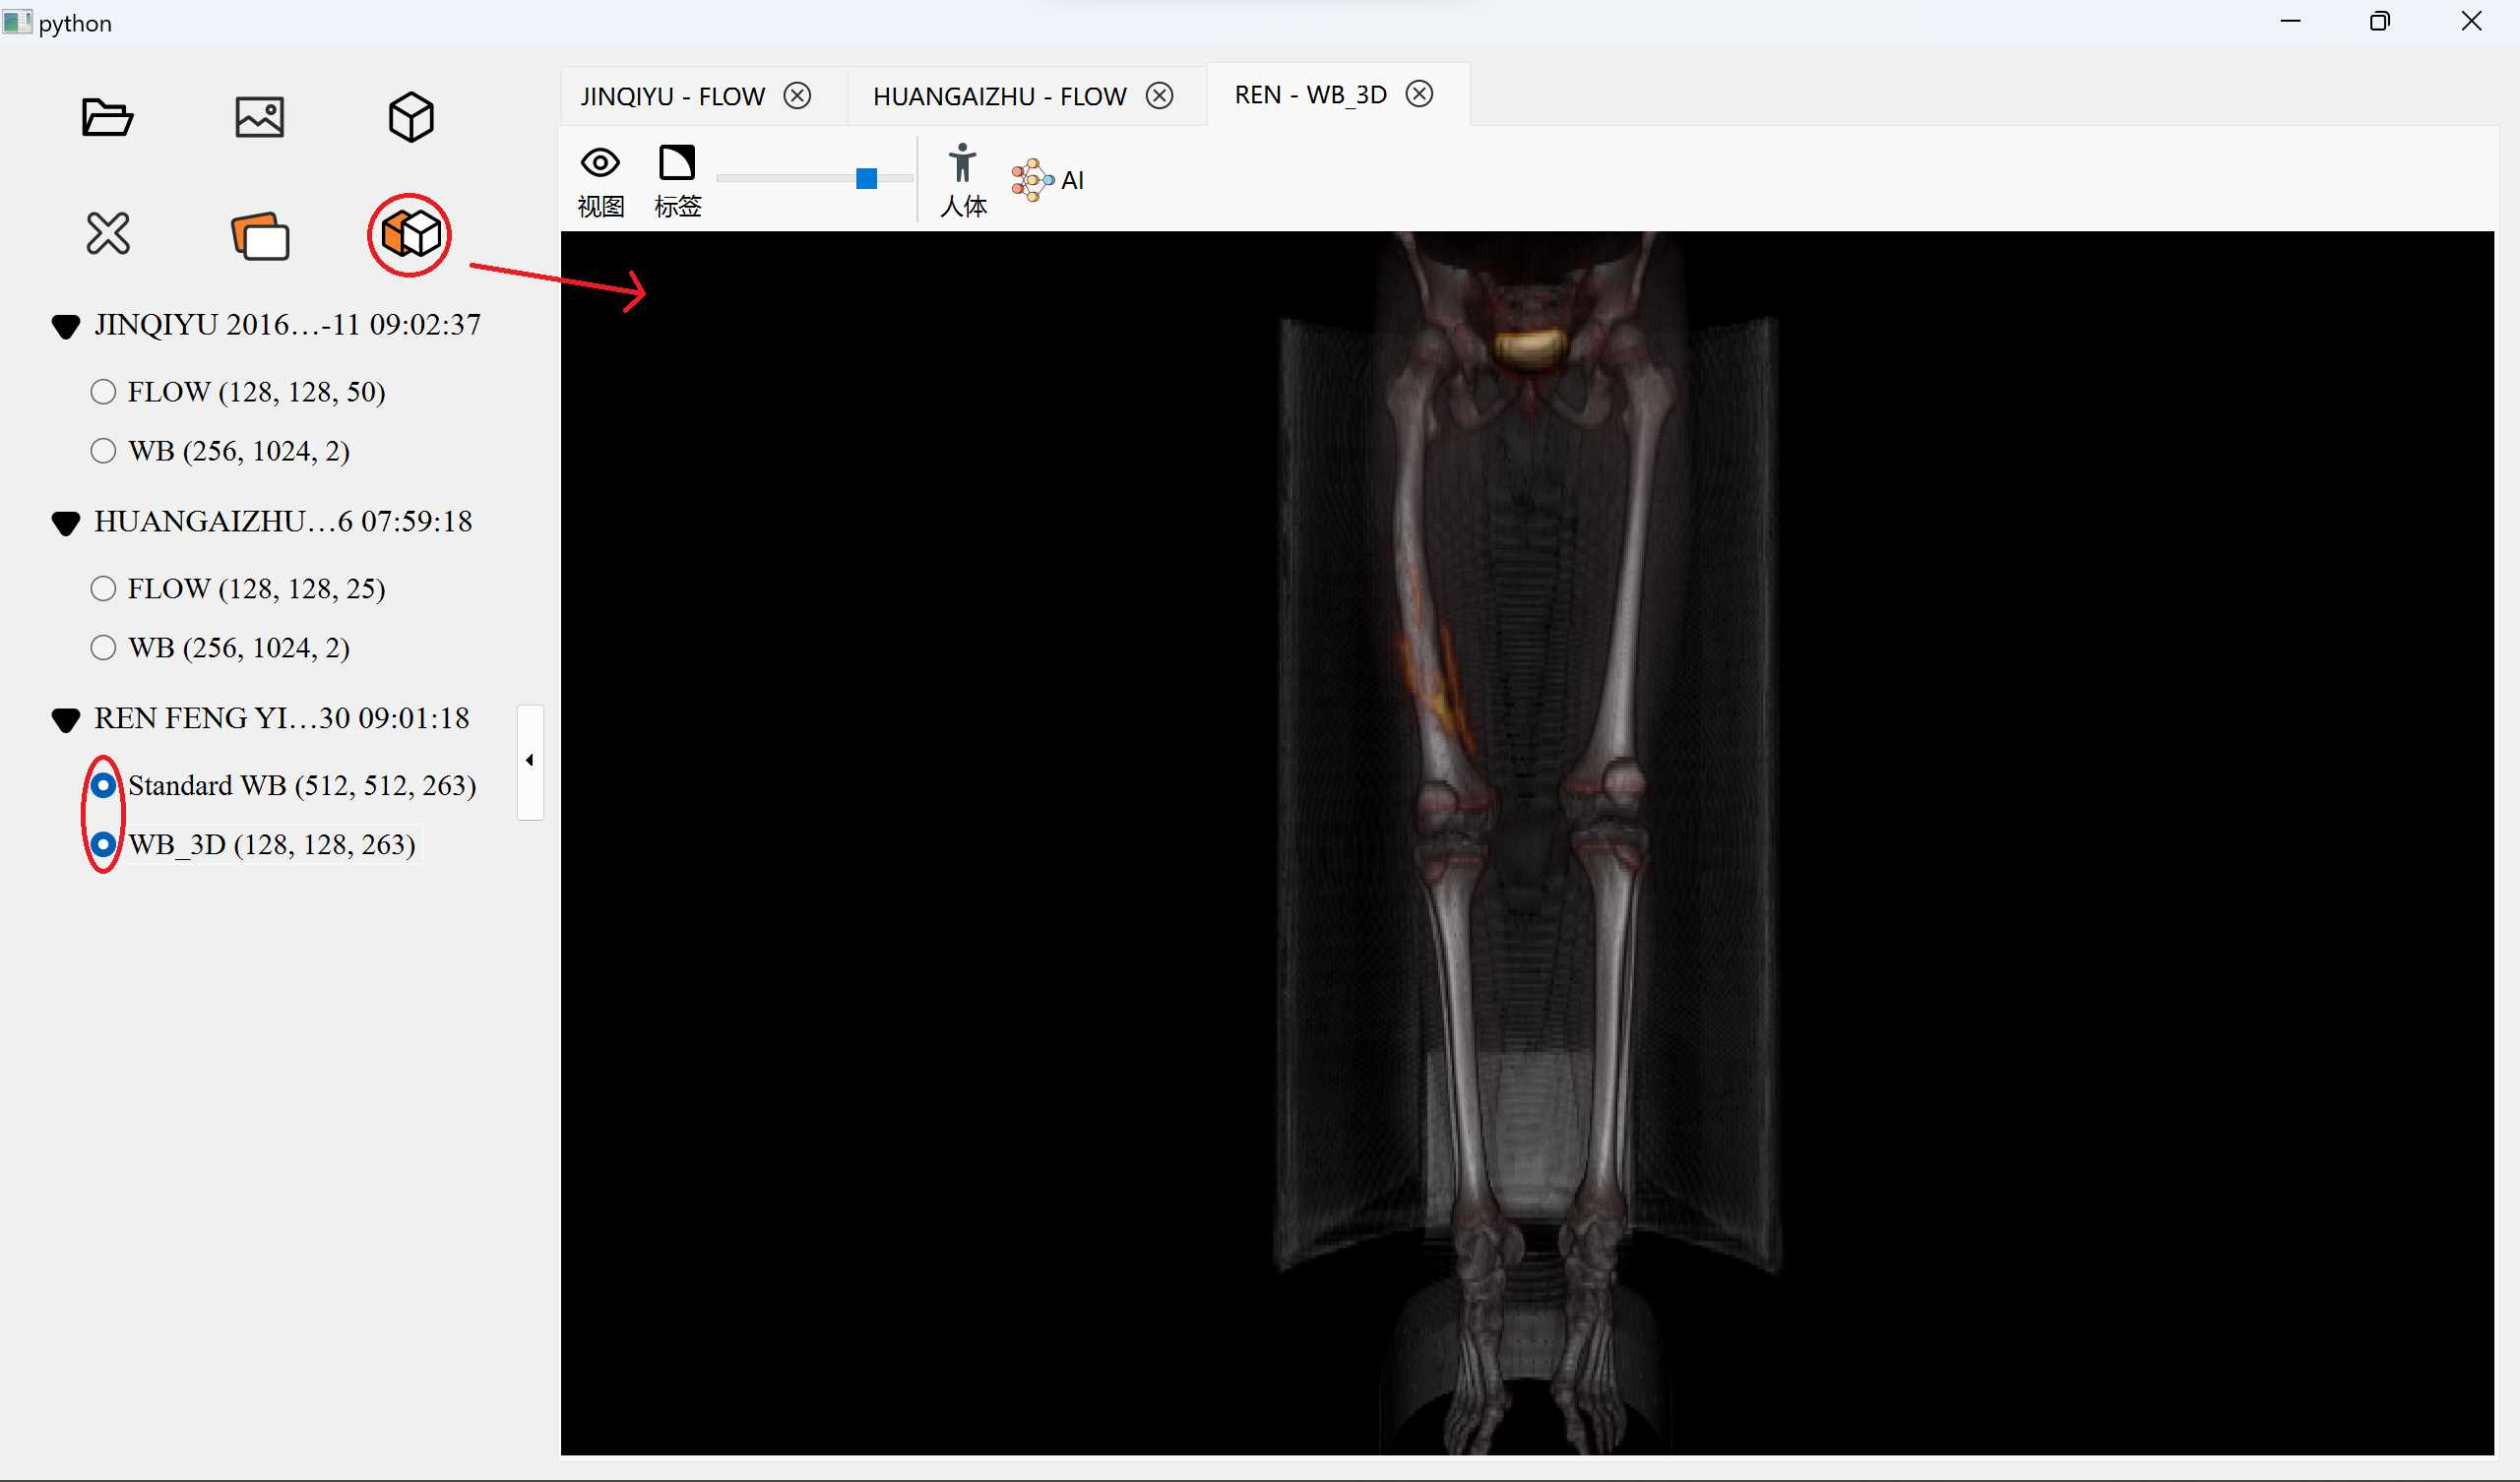
\includegraphics[width=0.49\textwidth]{figures/chap05_example04_vis.jpg}
    \label{fig:chap05_example04_vis}
  }
  \caption{可视化方法}\label{fig:chap05_example_vis}
\end{figure}

如图\ref{fig:chap05_example01_open}所示,通过在侧边导航栏顶部的“打开文件”功能按钮,可以在启动的文件选择窗口中依次打开患者A、患者B和患者C的DICOM医学影像文件。影像文件被打开并成功解析后,结果在侧边导航栏中清晰地展示了出来。

如图\ref{fig:chap05_example02_vis}所示,通过选中患者A的动态骨显像并点击“二维影像展示”按钮,从而呈现了患者A膝部的二维可视化影像。图\ref{fig:chap05_example03_vis}则展现了类似操作过程,勾选患者B的动态骨显像并点击相同的功能按钮,实现了髋部影像的二维可视化。随后,使用可视化区域顶部的影像分析工具。通过调整影像的对比度,以获得更清晰细致的可视化效果。在此基础上,灵活地切换不同的切片,搜索并定位到最合适的影像切片。最后,移动蓝色十字光标至特定区域,以查看相应的影像值,为进一步的分析和评估提供关键信息。

\begin{figure}[htbp]
  \centering
  \subfloat[膝部动态骨显像自动诊断]{
    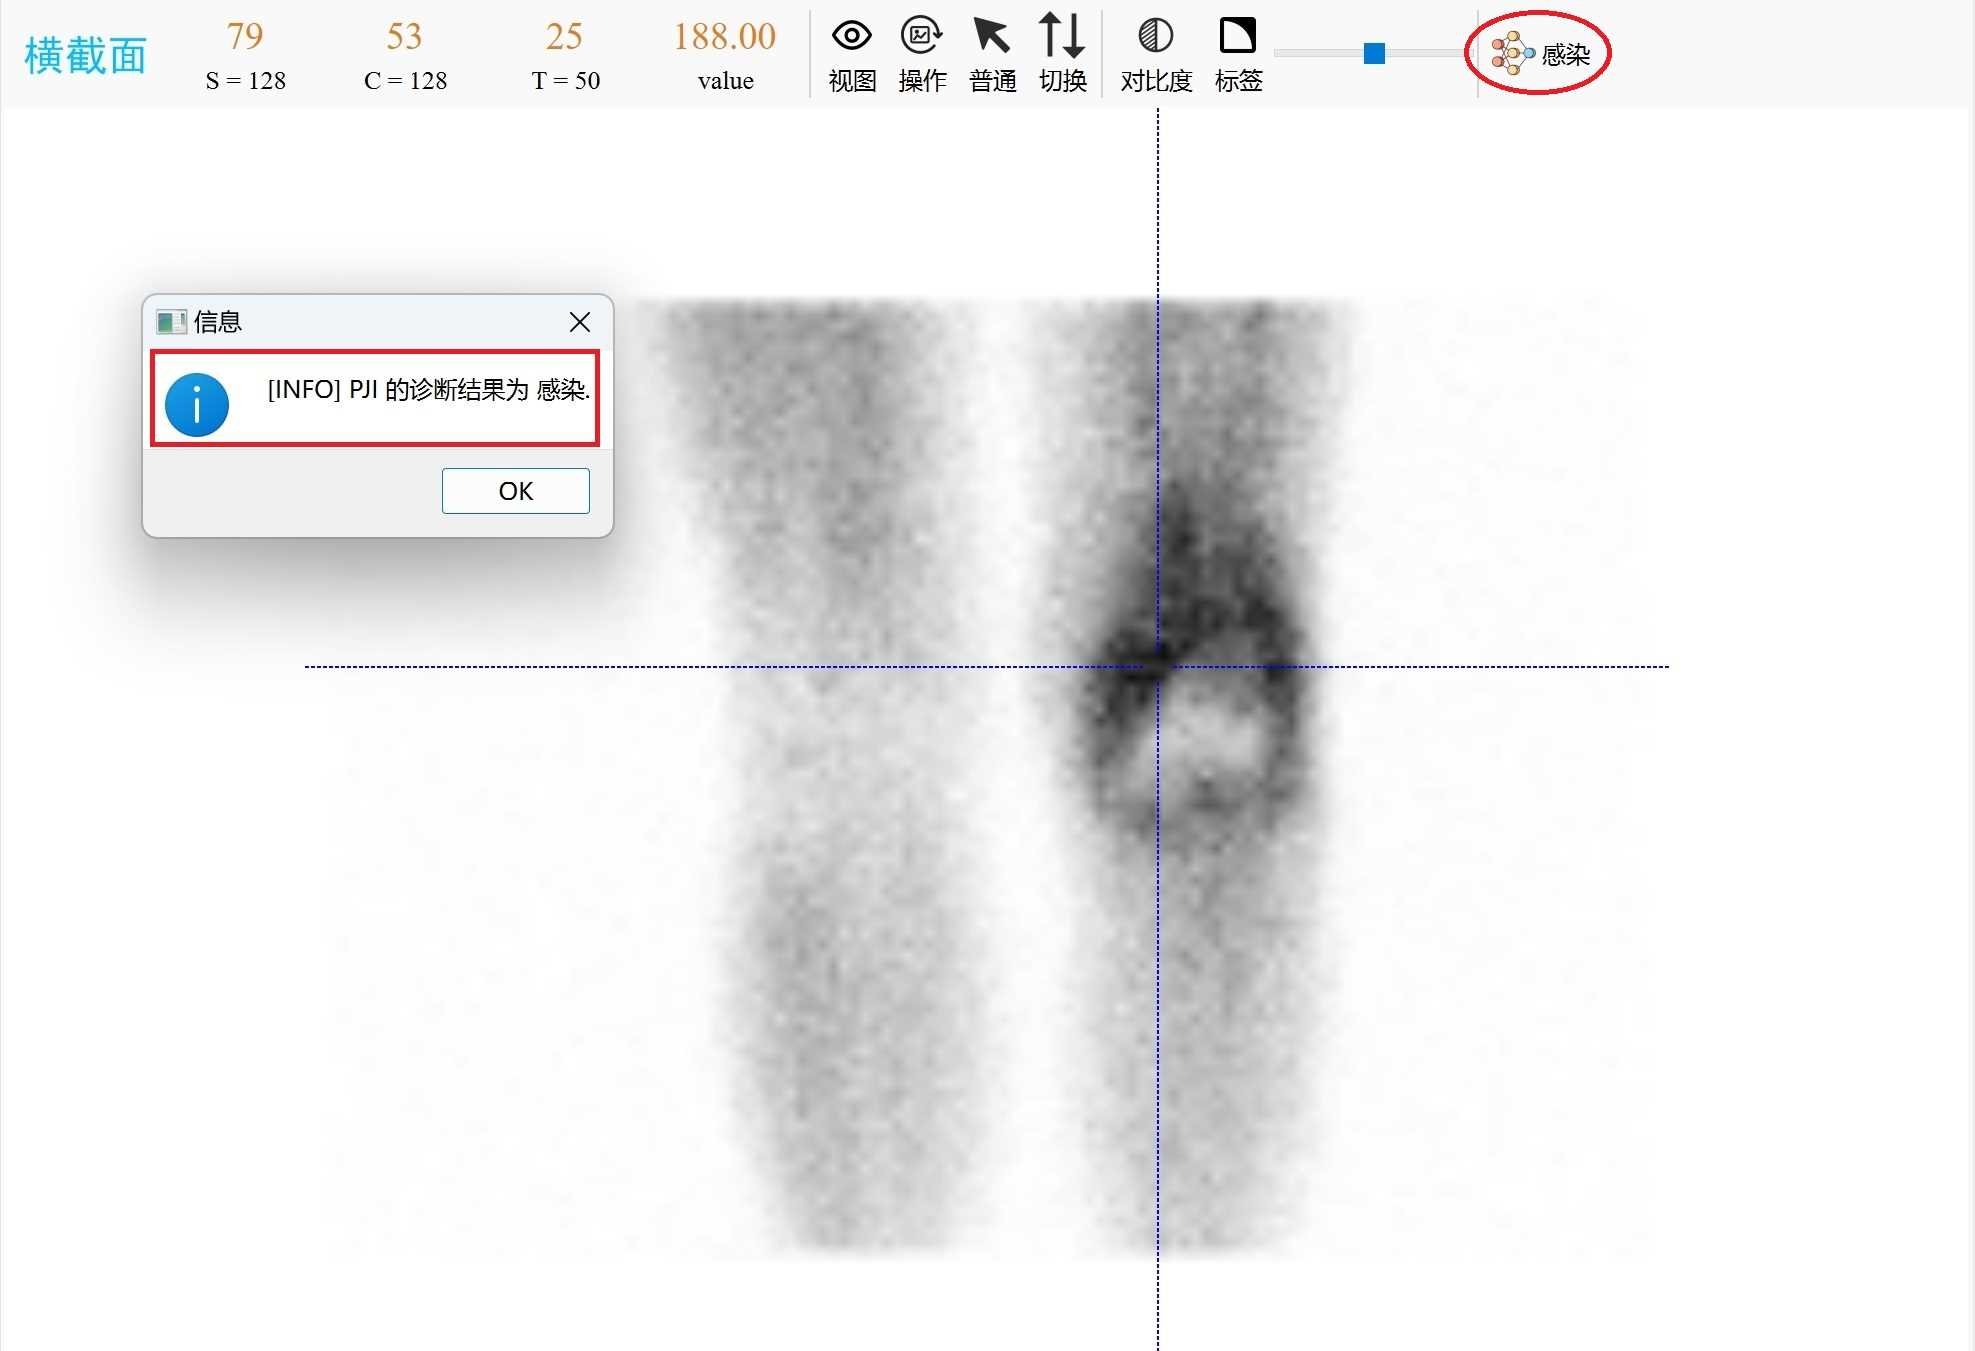
\includegraphics[width=0.475\textwidth]{figures/chap05_example_result1.jpg}
    \label{fig:chap05_example_result1}
  }
  \subfloat[髋部动态骨显像自动诊断]{
    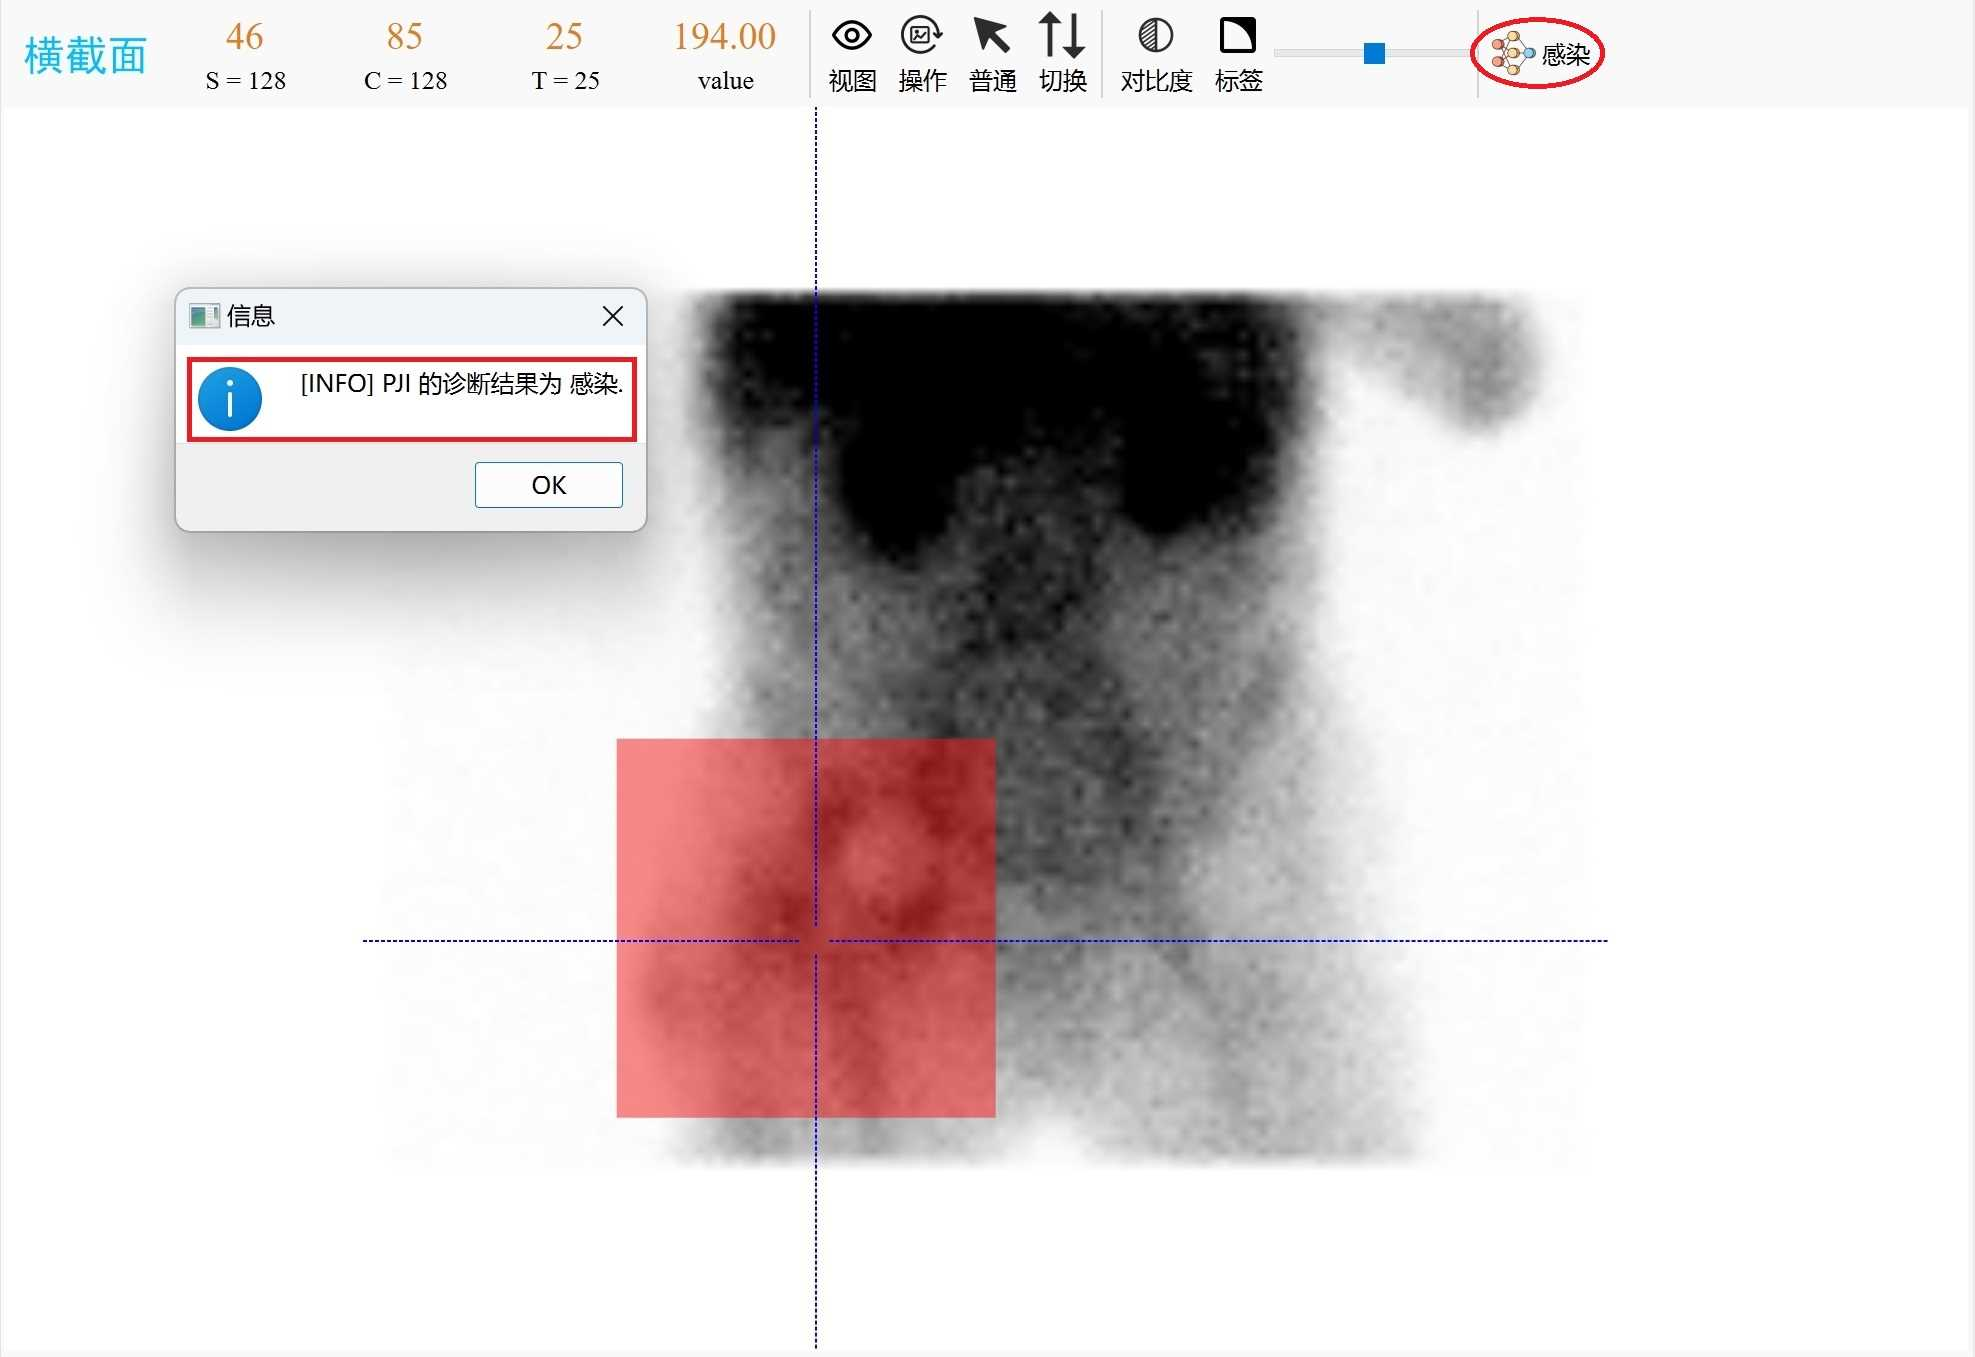
\includegraphics[width=0.475\textwidth]{figures/chap05_example_result2.jpg}
    \label{fig:chap05_example_result2}
  }
  \newline
  \newline
  \subfloat[下肢PET/CT自动诊断]{
    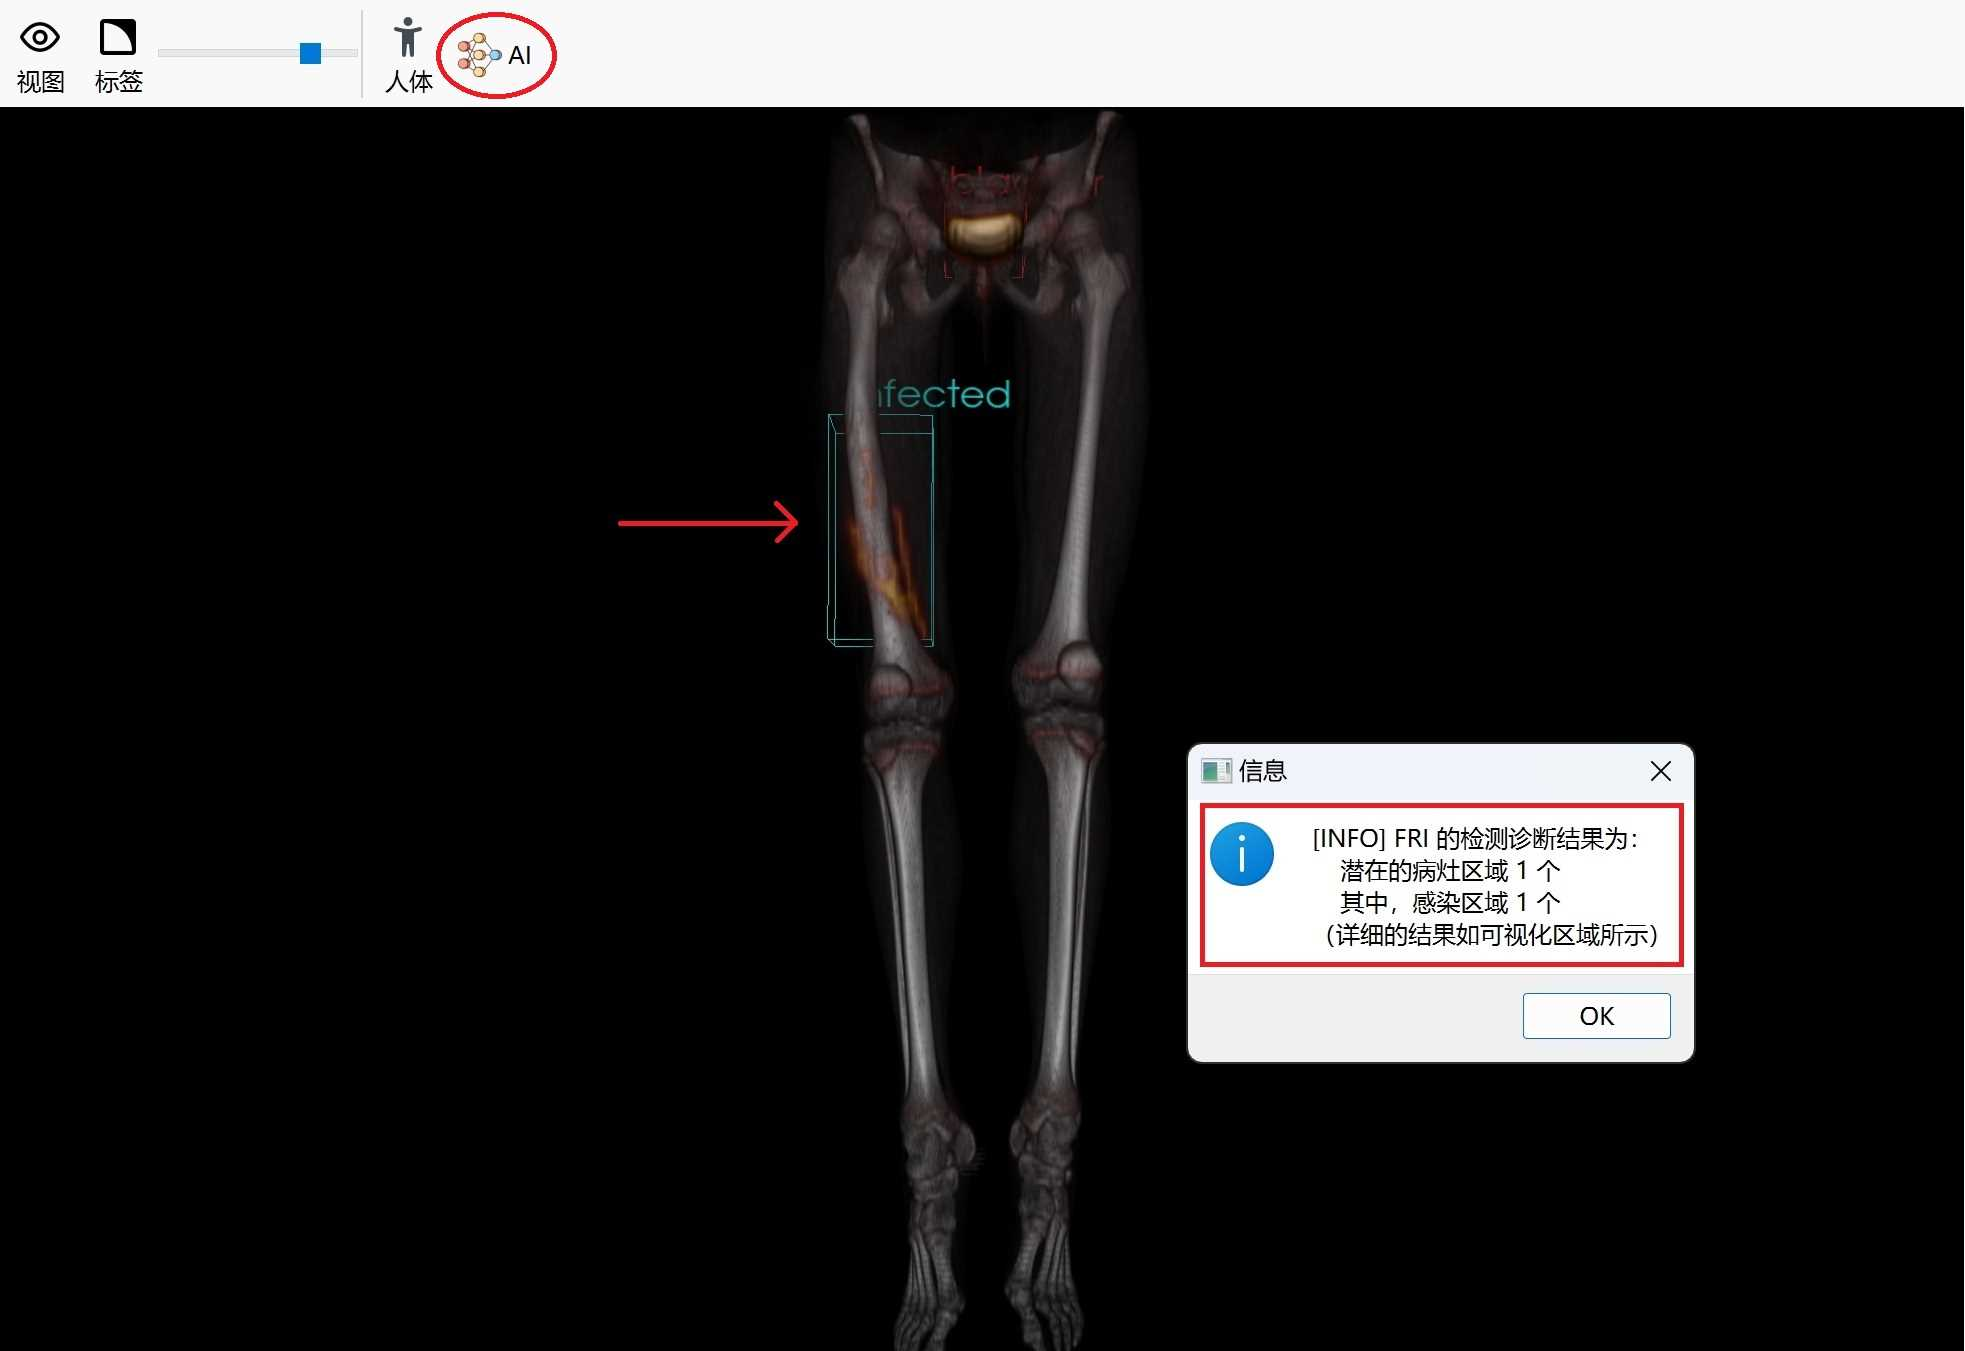
\includegraphics[width=0.475\textwidth]{figures/chap05_example_result3.jpg}
    \label{fig:chap05_example_result3}
  }
  \subfloat[PET/CT检测到的感染病灶]{
    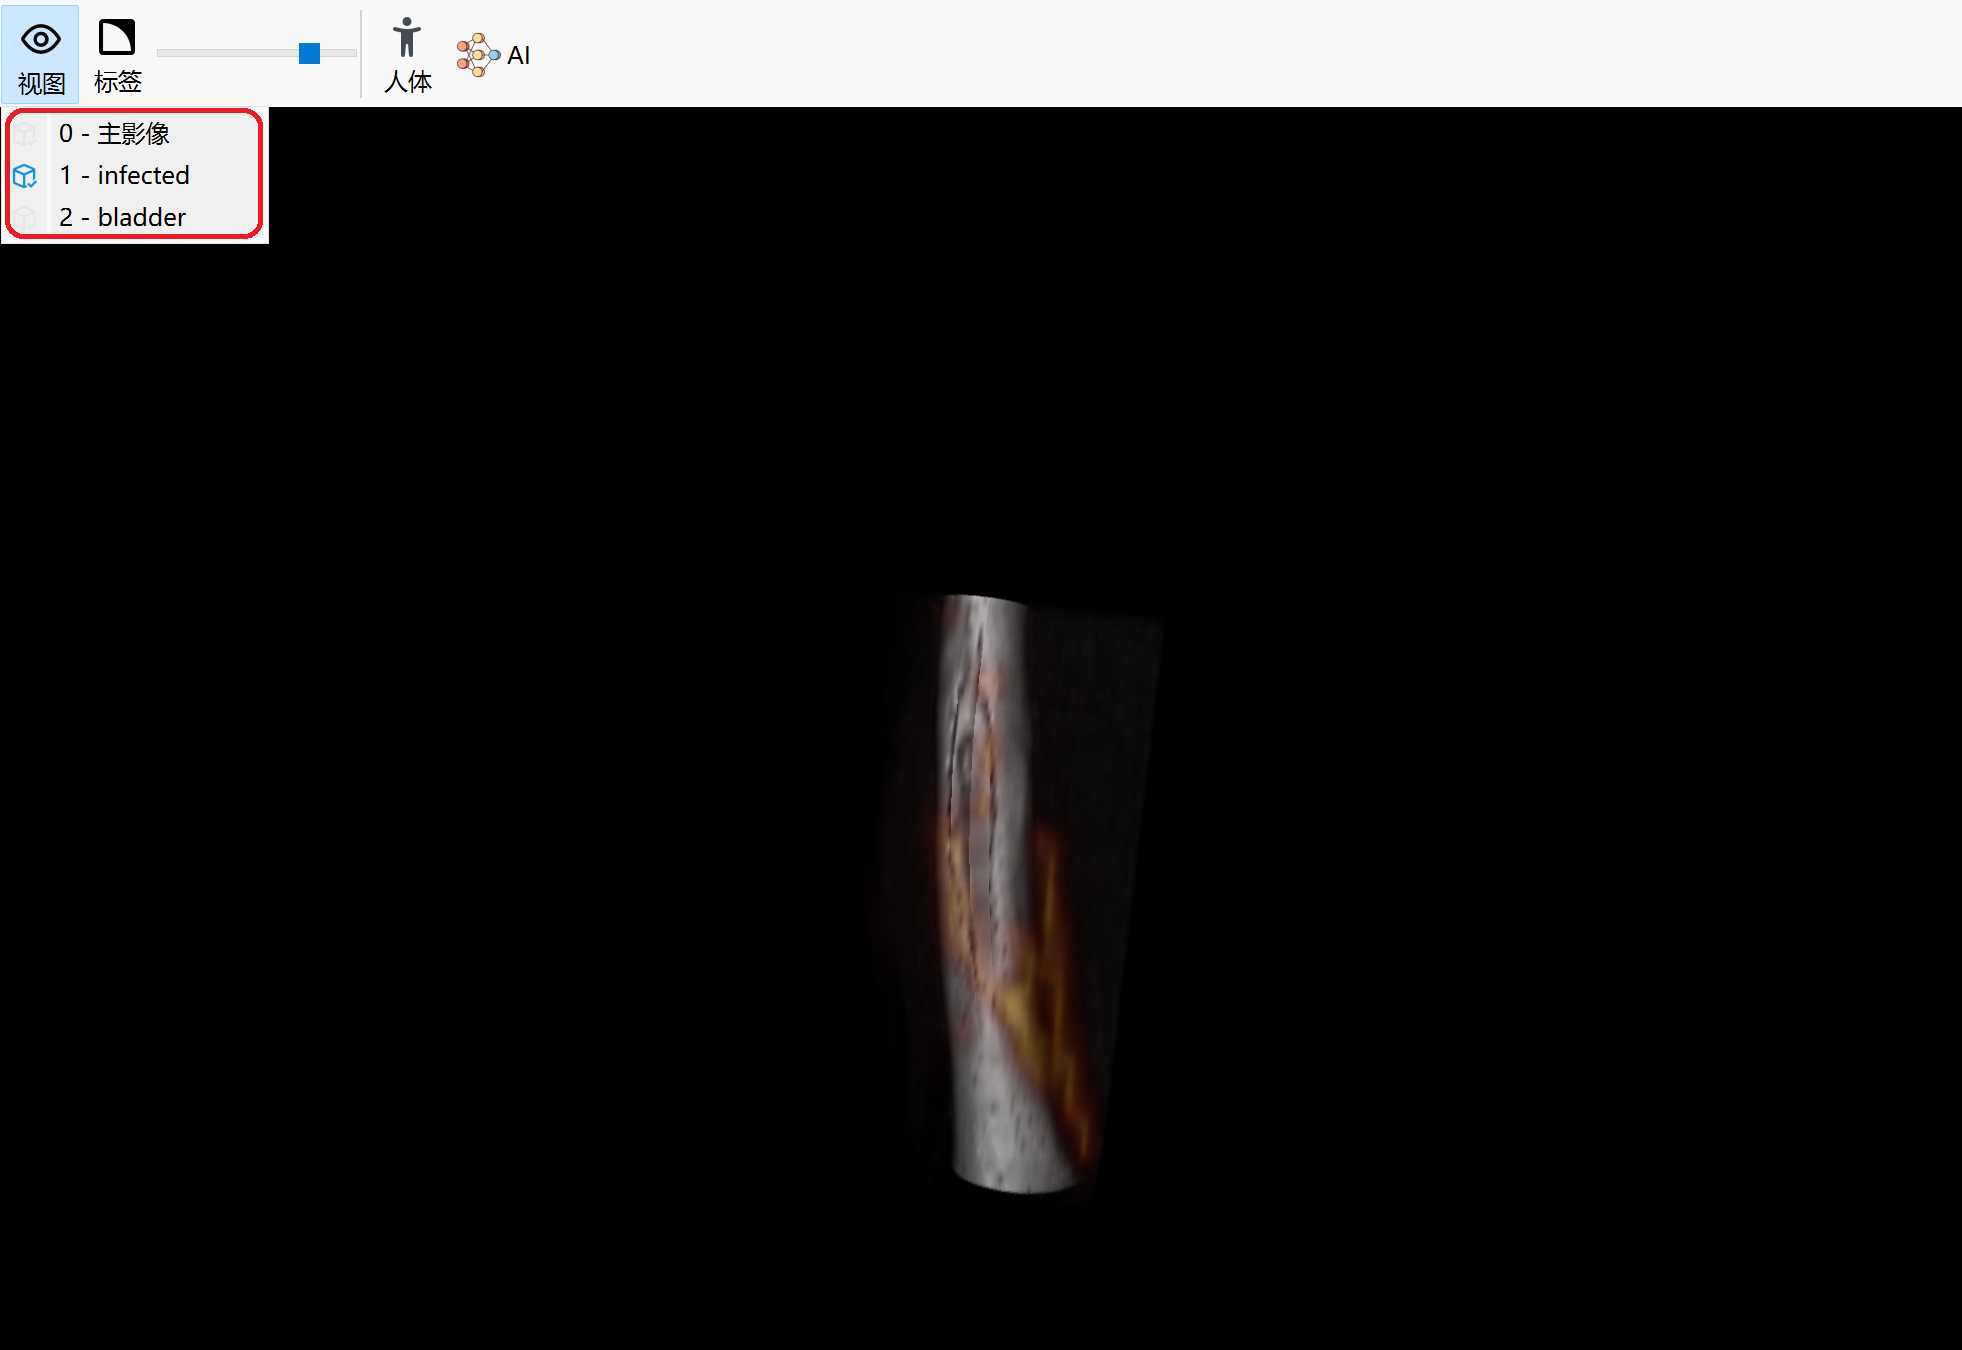
\includegraphics[width=0.475\textwidth]{figures/chap05_example_result4.jpg}
    \label{fig:chap05_example_result4}
  }
  \caption{自动诊断方法}
  \label{fig:chap05_example_diagnose}
\end{figure}


通过可视化区域顶部工具栏最右侧的AI功能按钮,可以激活辅助诊断模块的自动诊断功能,并获得基于深度学习方法生成的辅助诊断建议。图\ref{fig:chap05_example_result1}所展示的是患者A的案例,辅助诊断结果建议患者存在假体关节感染的情况。同时,图\ref{fig:chap05_example_result2}中以透明红色矩形标识了患者B髋部中的感兴趣区域,并表明了患者B存在假体关节感染的诊断建议。

图\ref{fig:chap05_example04_vis}展现了患者C的PET和CT影像数据,通过选中并点击“三维影像融合”按钮后,得到的下肢立体融合影像的可视化图。此后,利用影像分析工具可以对该立体影像进行缩放和旋转操作,以便对特定感兴趣的区域进行详细的观察和分析。点击AI辅助诊断按钮后,如图\ref{fig:chap05_example_result3}所呈现的,患者C被智能辅助诊断为存在一个感染区域,并且该区域在患者C的右股骨处被一个青色立体框所标记。最后借助于视图按钮,还能够从不同角度观察并分析感染区域的影像数据,如图\ref{fig:chap05_example_result4}所示。

通过对三个具体病例的详细展示和分析,提供的辅助诊断建议与经验丰富的医生所作出的诊断高度一致。这表明本章所介绍的自动诊断与可视化方法,不仅赋予了医生一个实用的影像分析工具,还可以通过整合先进的深度学习技术提出极具参考价值的辅助诊断建议。

\section{本章小结}

本章提出了一种用于骨科相关感染的自动诊断和可视化方法。此方法结合了前两章提出的人工关节感染辅助诊断框架与骨折相关感染的检测与诊断框架,以便进行对动态骨扫描和PET/CT影像的自动化处理和分析。同时,本方法还包含了从文件读取解析到医学影像的各种可视化,以及涵盖多项分析工具的影像分析,实现对医学影像中潜在病灶的定位与分析。本章最后通过三个真实案例的分析,验证了提出的辅助诊断建议与患者真实情况之间基本一致。这证明了本章方法,不仅为用户提供了一个全面而高效的可视化交互和分析工具,而且有助于促进医生的临床决策和提高准确性。